\documentclass[12pt, a4paper]{article}

% --- Preamble: Load Packages ---
\usepackage[utf8]{inputenc}
\usepackage[T1]{fontenc}
\usepackage[margin=1in]{geometry} % Sets 1-inch margins
\usepackage{amsmath, amssymb, amsthm} % Core math packages
\usepackage{graphicx} % For figure placeholders
\usepackage{booktabs} % For professional tables
\usepackage[hidelinks]{hyperref} % For clickable links
\usepackage{cite} % For bibliography
\usepackage{setspace} % For line spacing adjustments
\usepackage{enumitem} % For customizing lists

% --- Spacing Adjustments ---
\setlength{\parindent}{0pt} % No paragraph indentation
\setlength{\parskip}{1.5ex} % Vertical space between paragraphs
\setlist{itemsep=0.5ex} % Space between list items

% --- Theorem Environments (for a 'math note' style) ---
\theoremstyle{definition}
\newtheorem{definition}{Definition}[section]
\newtheorem{example}{Example}[section]

\theoremstyle{plain}
\newtheorem{theorem}{Theorem}[section]
\newtheorem{corollary}{Corollary}[section]

\theoremstyle{remark}
\newtheorem{remark}{Remark}[section]

% --- Title ---
\title{Set Theory and Probability I}
\author{Mahbubur Rahman Khan}
\date{\today}

% --- Document Body ---
\begin{document}

\maketitle

% --- Abstract ---
\begin{abstract}
    This note presents fundamental concepts in Set Theory and Probability Theory. Material from CSE422 class (taught by Md. Shahriar Karim, Assistant Professor, North South University) lectures is enhanced with definitions, theorems, examples, and proofs from faculty notes \cite{faculty_set, faculty_prob} and textbooks by Ross \cite{ross} and Chan \cite{chan}. Topics include set operations, cardinality, probability spaces, axioms, corollaries, probability assignment (pmf/pdf), measure zero sets, and conditional probability.
\end{abstract}

\thispagestyle{empty}
\tableofcontents
\newpage
\setcounter{page}{1}

% --- Section 1: Set Theory ---
\section{Set Theory}

Set theory forms the fundamental language and mathematical basis for understanding probability. We begin by defining the core concepts.

\subsection{Sets and Elements}

A \textbf{set} is a collection of distinct objects, considered as an entity in itself. The objects within the set are called its \textbf{elements} or members. Sets are typically denoted by capital letters (e.g., $A, B, S$) and their elements by lowercase letters or symbols.

\begin{definition}[Set]
    A \textbf{set} is a collection of distinct elements. We often denote a set by listing its elements within curly braces \cite{faculty_set, chan}.
    $$A = \{\xi_1, \xi_2, ..., \xi_n\}$$
    where $\xi_i$ is the $i$-th element in the set.
\end{definition}

\begin{remark}
    The elements in a set are \textbf{distinct} (no repetitions) and \textbf{unordered} (the order in which elements are listed does not matter).
\end{remark}

\begin{example}
    \begin{itemize}
        \item $A = \{2, 7, 9\}$ is a finite set of numbers.
        \item $B = \{\text{apple, orange, pear}\}$ is a finite set of objects.
        \item $C = \{2, 4, 6, 8, ...\}$ is an infinite set (the set of positive even integers).
    \end{itemize}
\end{example}

\begin{definition}[Element Membership]
    If an object $\xi$ is an element of a set $A$, we write $\xi \in A$. If $\xi$ is not an element of $A$, we write $\xi \notin A$.
\end{definition}

\subsection{Describing Sets}

Sets can be described explicitly by listing elements or implicitly using properties.

\begin{definition}[Set Builder Notation]
    A set can be defined by specifying a property that its elements must satisfy.
    $$A = \{x \mid P(x)\}$$
    This reads as "A is the set of all elements $x$ such that property $P(x)$ is true."
\end{definition}

\begin{example}
    \begin{itemize}
        \item $A = \{1, 2, 3, 4, 5, 6, 7, 8, 9\}$ can be written as $A = \{x \mid x \in \mathbb{Z}^+ \text{ and } 1 \le x \le 9\}$.
        \item The set of even integers can be written as $E = \{x \mid x = 2k \text{ for some integer } k\}$.
    \end{itemize}
\end{example}

\subsection{Fundamental Set Concepts}

\begin{definition}[Set Equality]
    Two sets $A$ and $B$ are \textbf{equal} ($A = B$) if and only if they contain exactly the same elements \cite{faculty_set, ross}.
\end{definition}

\begin{definition}[Cardinality]
    The \textbf{cardinality} of a finite set $A$, denoted $|A|$, is the number of distinct elements in the set \cite{faculty_set}.
\end{definition}

\begin{example}
    For $A = \{2, 7, 9\}$, $|A| = 3$.
\end{example}

\begin{definition}[Universal Set ($\Omega$)]
    In a particular context, the \textbf{Universal Set} ($\Omega$ or $S$) is the set containing all possible elements under consideration \cite{faculty_set, chan}.
\end{definition}

\begin{definition}[Empty Set ($\emptyset$)]
    The \textbf{Empty Set} ($\emptyset$ or $\{\}$) is the unique set containing no elements \cite{faculty_set, ross}.
\end{definition}

\begin{definition}[Subset ($A \subseteq B$)]
    Set $A$ is a \textbf{subset} of set $B$ if every element of $A$ is also an element of $B$ \cite{chan}. If $A \subseteq B$ and $A \ne B$, then $A$ is a \textbf{proper subset} of $B$, denoted $A \subset B$.
\end{definition}

\begin{theorem}
    Two sets $A$ and $B$ are equal if and only if $A \subseteq B$ and $B \subseteq A$ \cite{chan}.
\end{theorem}

\subsection{Set Operations}

These operations allow us to combine or modify sets.

\begin{definition}[Union ($A \cup B$)]
    The \textbf{union} of sets $A$ and $B$ is the set containing all elements that are in $A$, or in $B$, or in both \cite{ross}.
    $$A \cup B = \{x \mid x \in A \text{ or } x \in B\}$$
\end{definition}

\begin{example}
    If $A = \{1, 2, 3\}$ and $B = \{3, 4, 5\}$, then $A \cup B = \{1, 2, 3, 4, 5\}$.
\end{example}

\begin{figure}[h!]
    \centering
    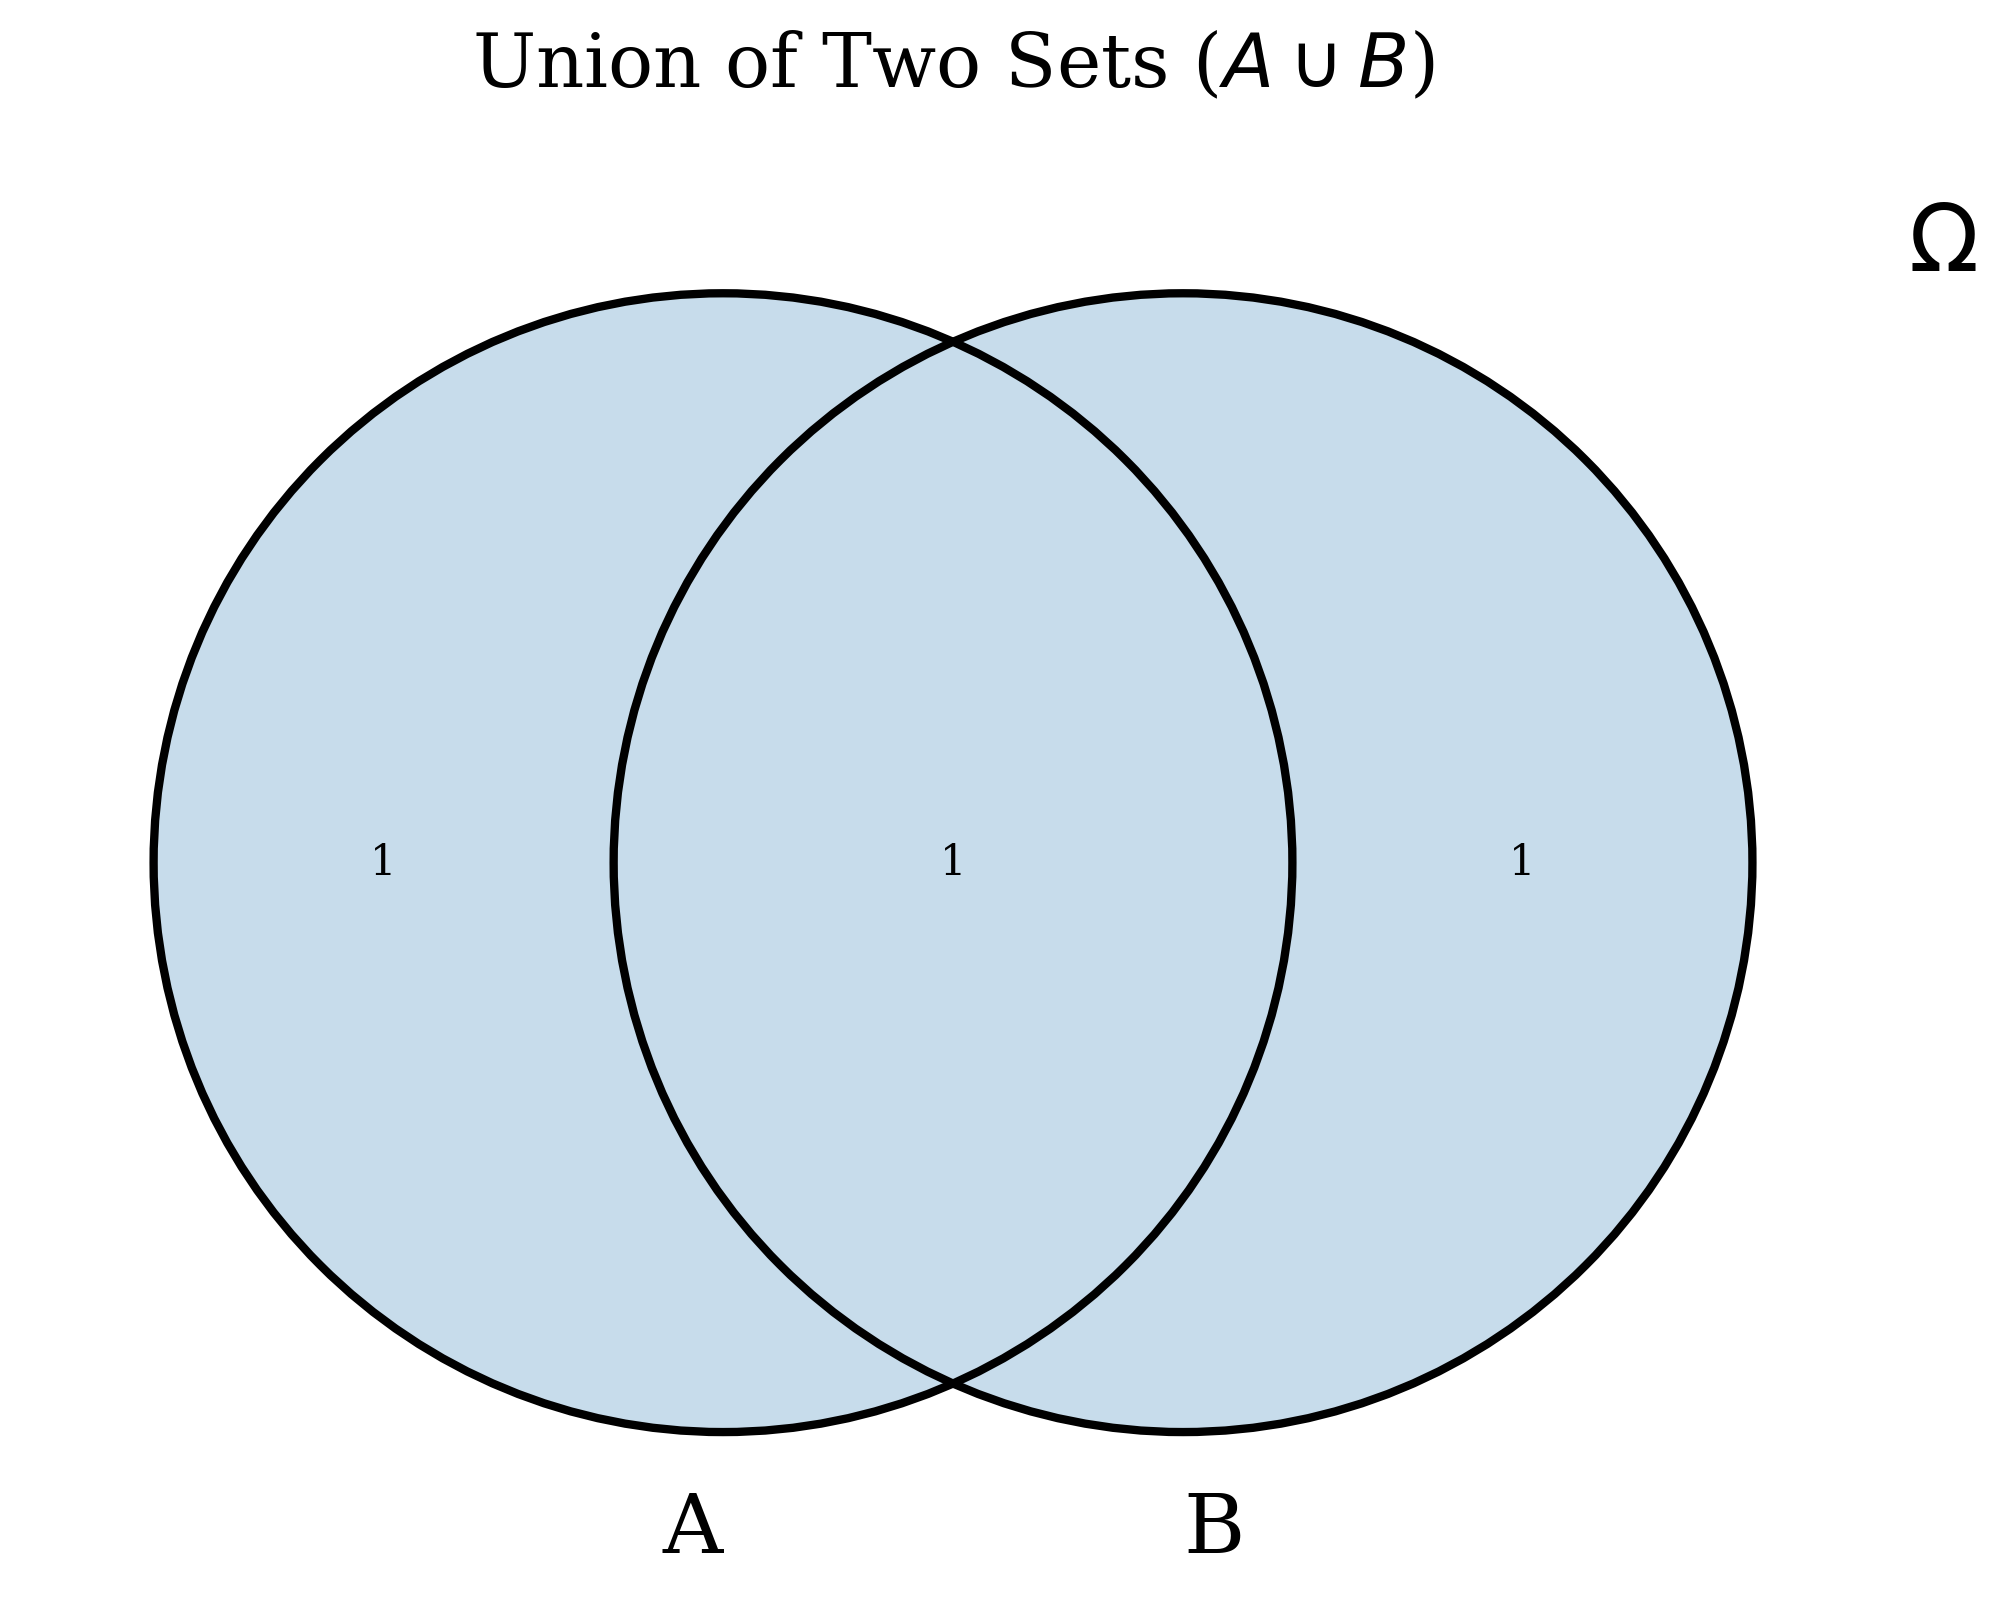
\includegraphics[width=0.6\textwidth]{figure_1_union.png}
    \caption{Venn Diagram for Union $A \cup B$.}
    \label{fig:union_venn}
\end{figure}

\begin{definition}[Intersection ($A \cap B$)]
    The \textbf{intersection} of sets $A$ and $B$ is the set containing all elements that are common to both $A$ and $B$ \cite{ross}.
    $$A \cap B = \{x \mid x \in A \text{ and } x \in B\}$$
\end{definition}

\begin{example}
    If $A = \{1, 2, 3\}$ and $B = \{3, 4, 5\}$, then $A \cap B = \{3\}$.
    If $C = \{1, 2\}$ and $D = \{3, 4\}$, then $C \cap D = \emptyset$.
\end{example}

\begin{figure}[h!]
    \centering
    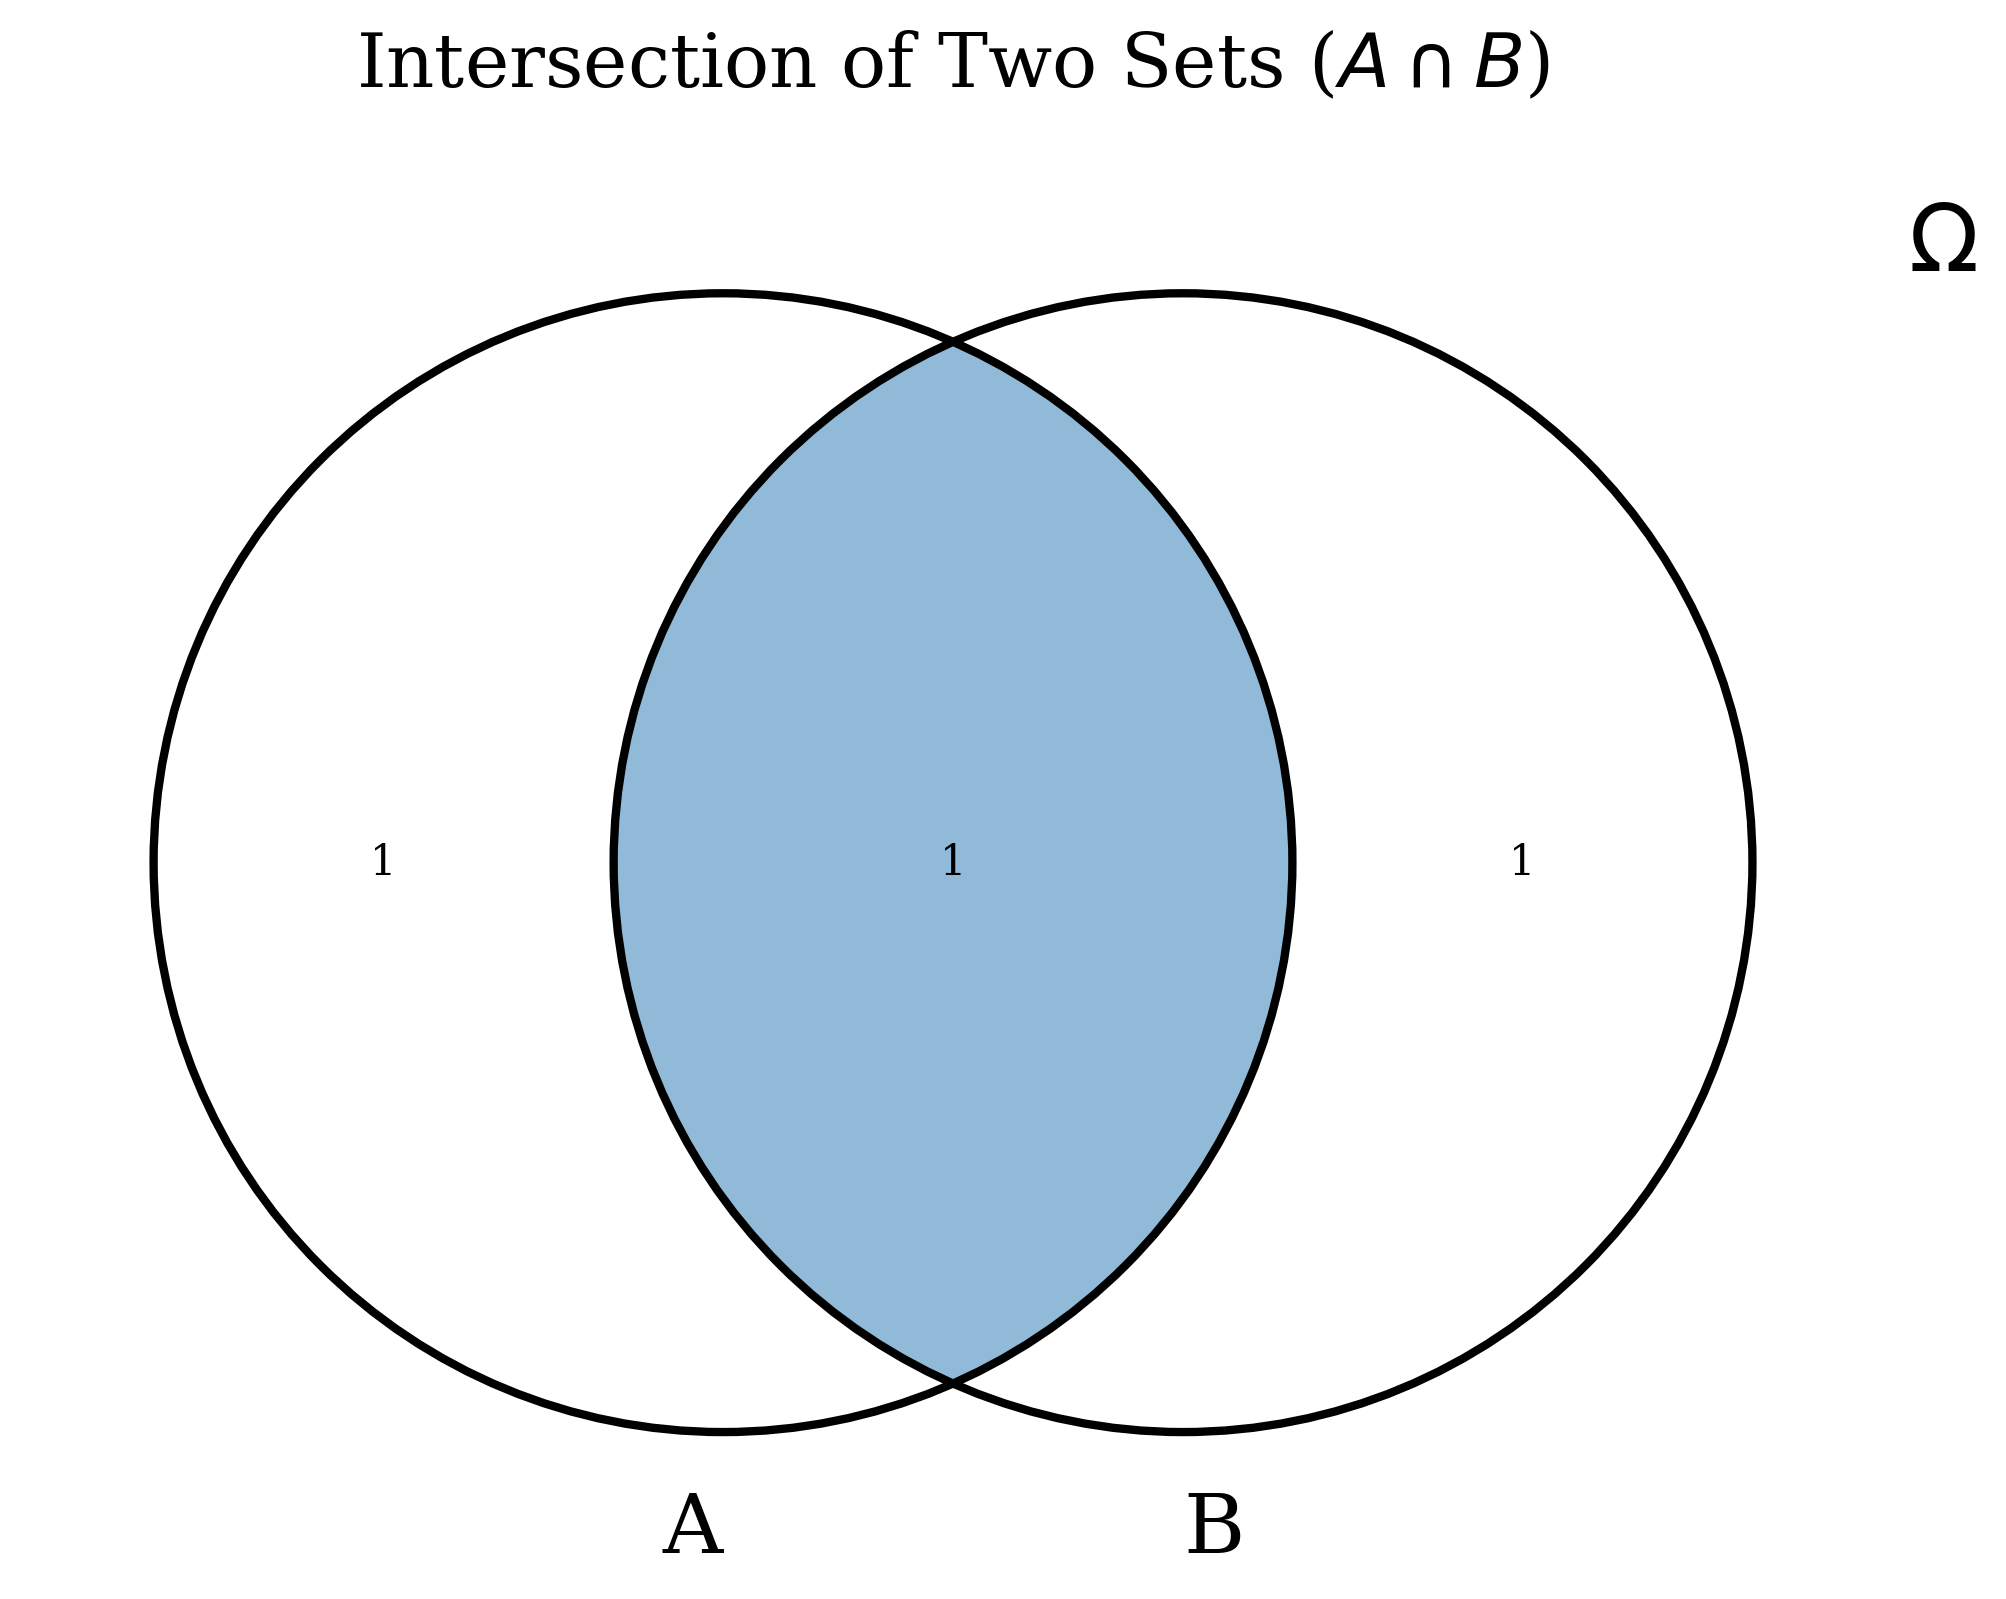
\includegraphics[width=0.6\textwidth]{figure_2_intersection.png}
    \caption{Venn Diagram for Intersection $A \cap B$.}
    \label{fig:intersection_venn}
\end{figure}

\begin{definition}[Complement ($A^c$ or $\bar{A}$)]
    Relative to a universal set $\Omega$, the \textbf{complement} of $A$ is the set of all elements in $\Omega$ that are \emph{not} in $A$ \cite{faculty_set, ross}.
    $$A^c = \{x \mid x \in \Omega \text{ and } x \notin A\}$$
\end{definition}

\begin{figure}[h!]
    \centering
    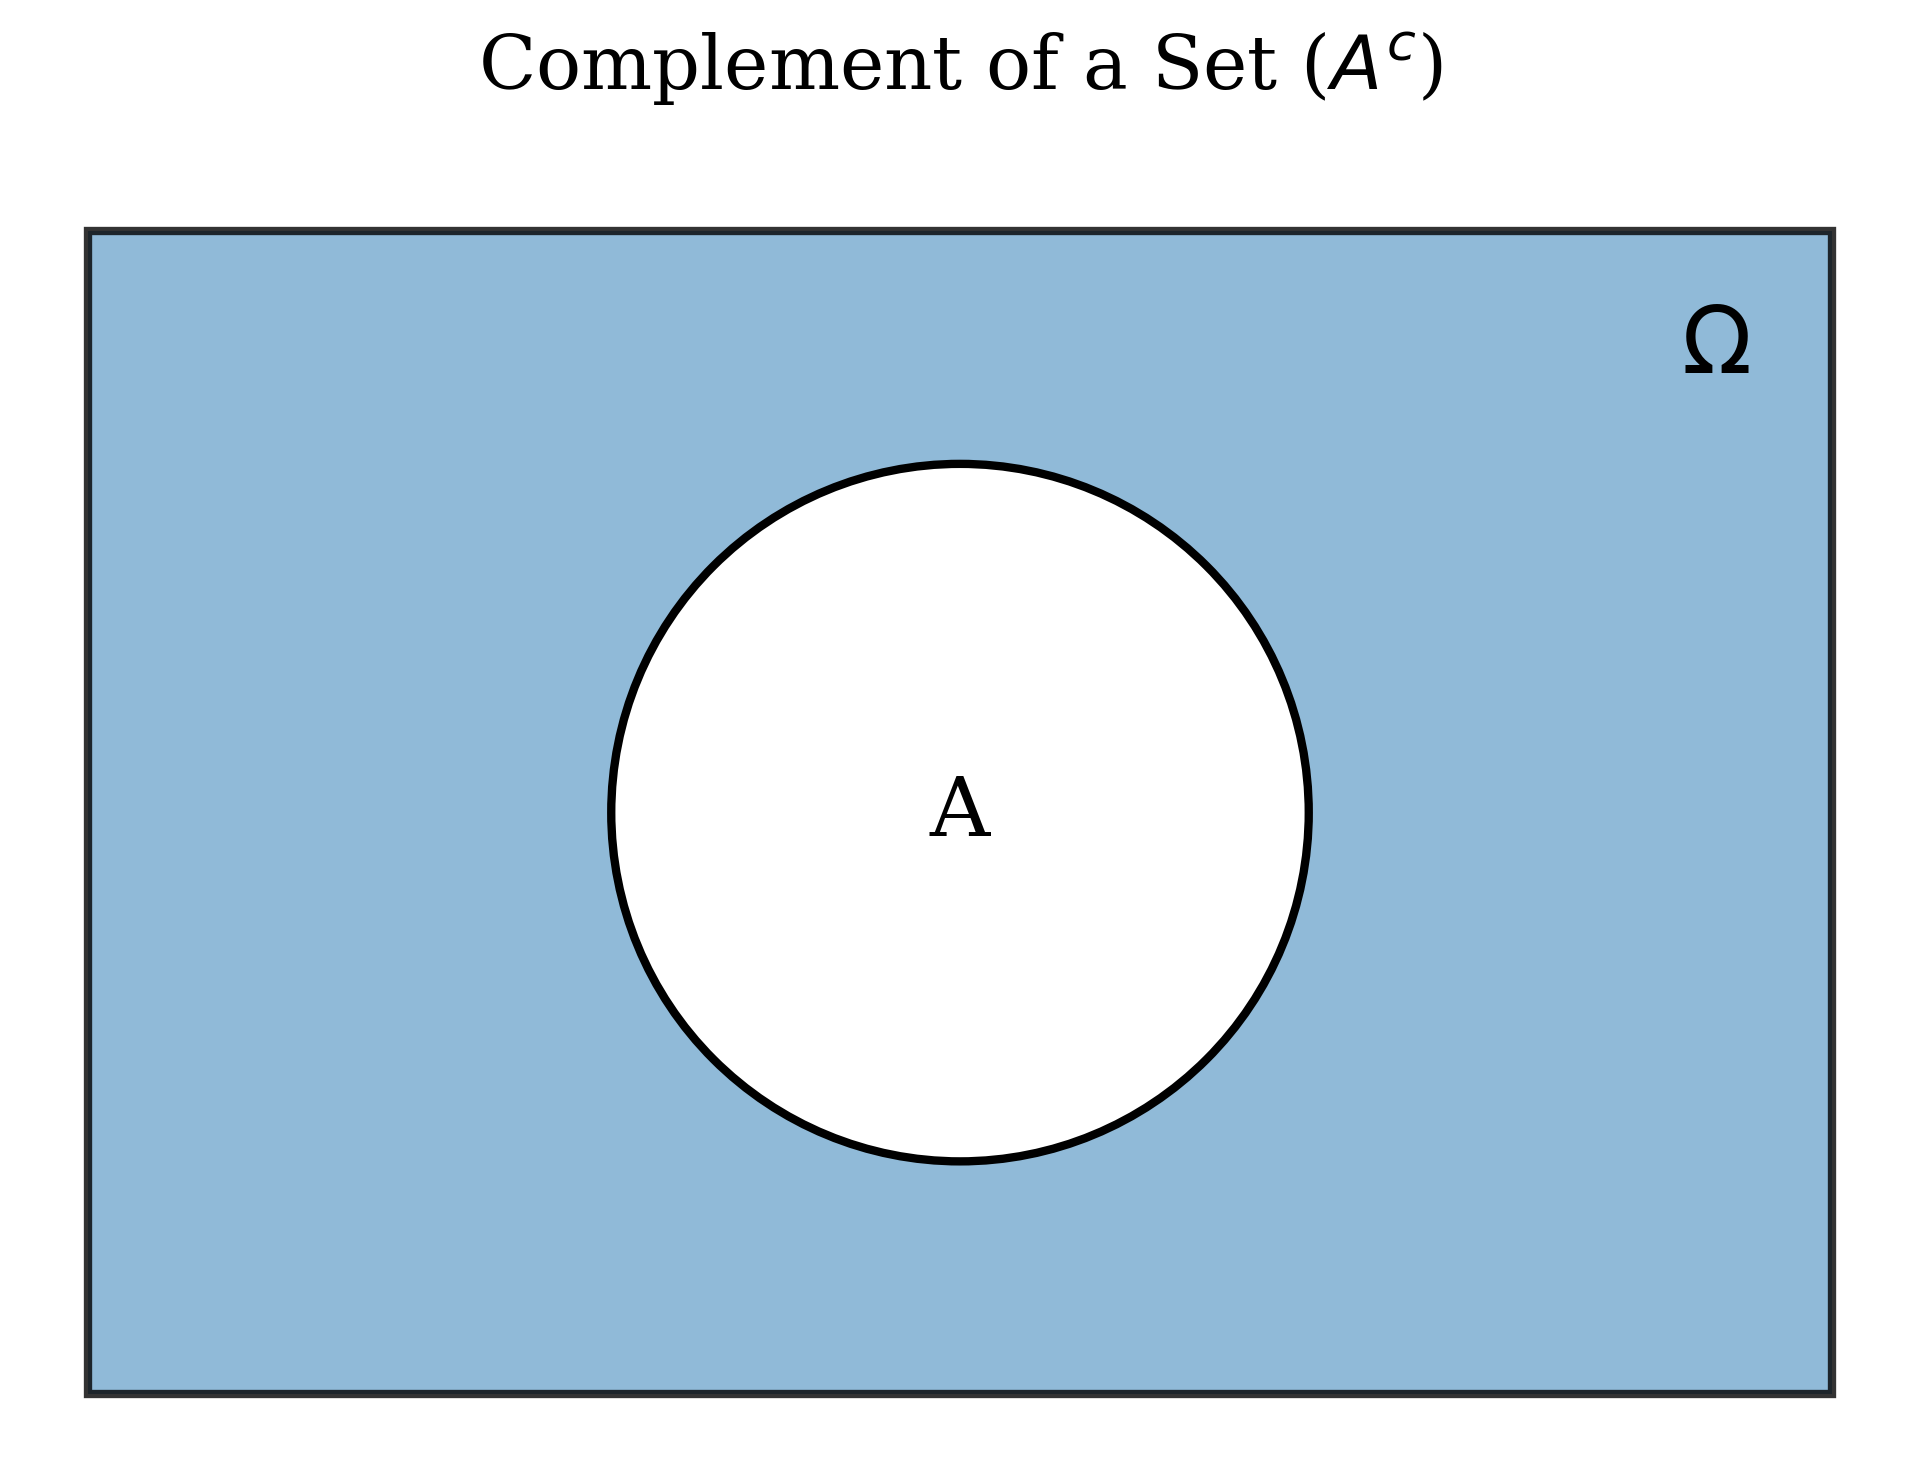
\includegraphics[width=0.6\textwidth]{figure_3_complement.png}
    \caption{Venn Diagram for Complement $A^c$.}
    \label{fig:complement_venn}
\end{figure}

\begin{definition}[Set Difference ($A \setminus B$)]
    The \textbf{difference} of sets $A$ and $B$ is the set containing all elements that are in $A$ but \emph{not} in $B$ \cite{faculty_set, chan}.
    $$A \setminus B = \{x \mid x \in A \text{ and } x \notin B\}$$
    Note that $A \setminus B = A \cap B^c$.
\end{definition}

\begin{figure}[h!]
    \centering
    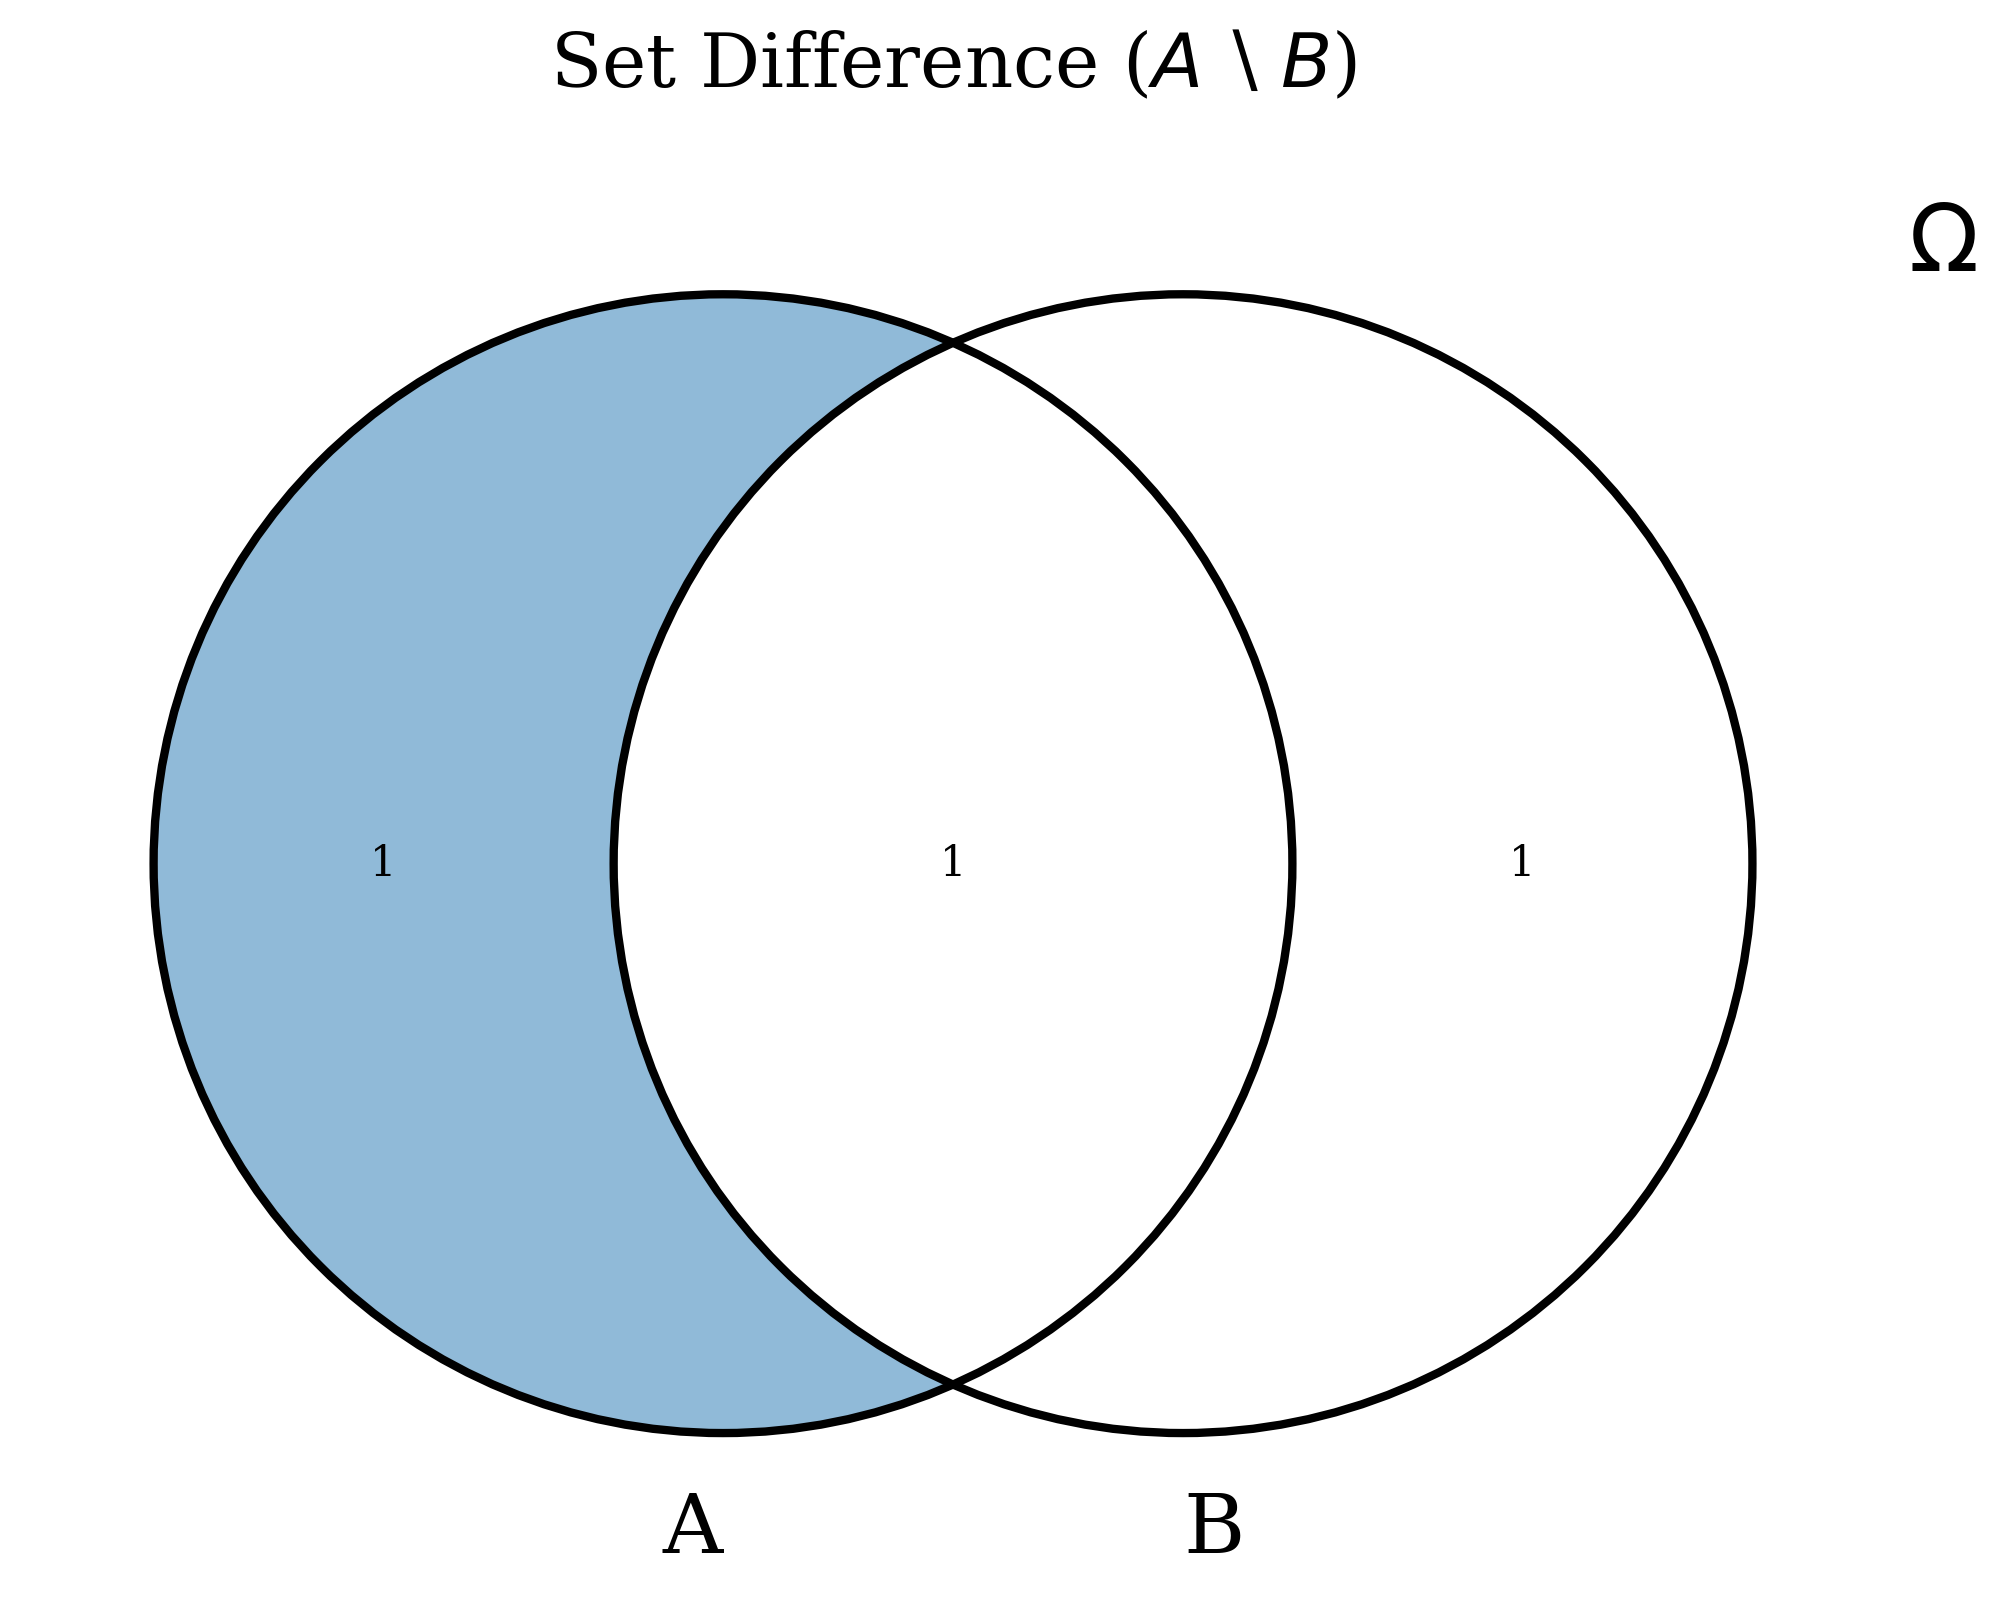
\includegraphics[width=0.6\textwidth]{figure_4_set_difference.png}
    \caption{Venn Diagram for Set Difference $A \setminus B$.}
    \label{fig:difference_venn}
\end{figure}

\subsection{Disjoint Sets and Partitions}

\begin{definition}[Disjoint Sets]
    Two sets $A$ and $B$ are \textbf{disjoint} (or mutually exclusive) if they have no elements in common, i.e., $A \cap B = \emptyset$ \cite{faculty_set, chan}.
\end{definition}

\begin{definition}[Partition]
    A collection of non-empty sets $\{A_1, ..., A_n\}$ forms a \textbf{partition} of a set $\Omega$ if \cite{faculty_set, chan}:
    \begin{enumerate}
        \item The sets are pairwise disjoint: $A_i \cap A_j = \emptyset$ for all $i \ne j$.
        \item The sets are collectively exhaustive: $\bigcup_{i=1}^n A_i = \Omega$.
    \end{enumerate}
\end{definition}

\begin{figure}[h!]
    \centering
    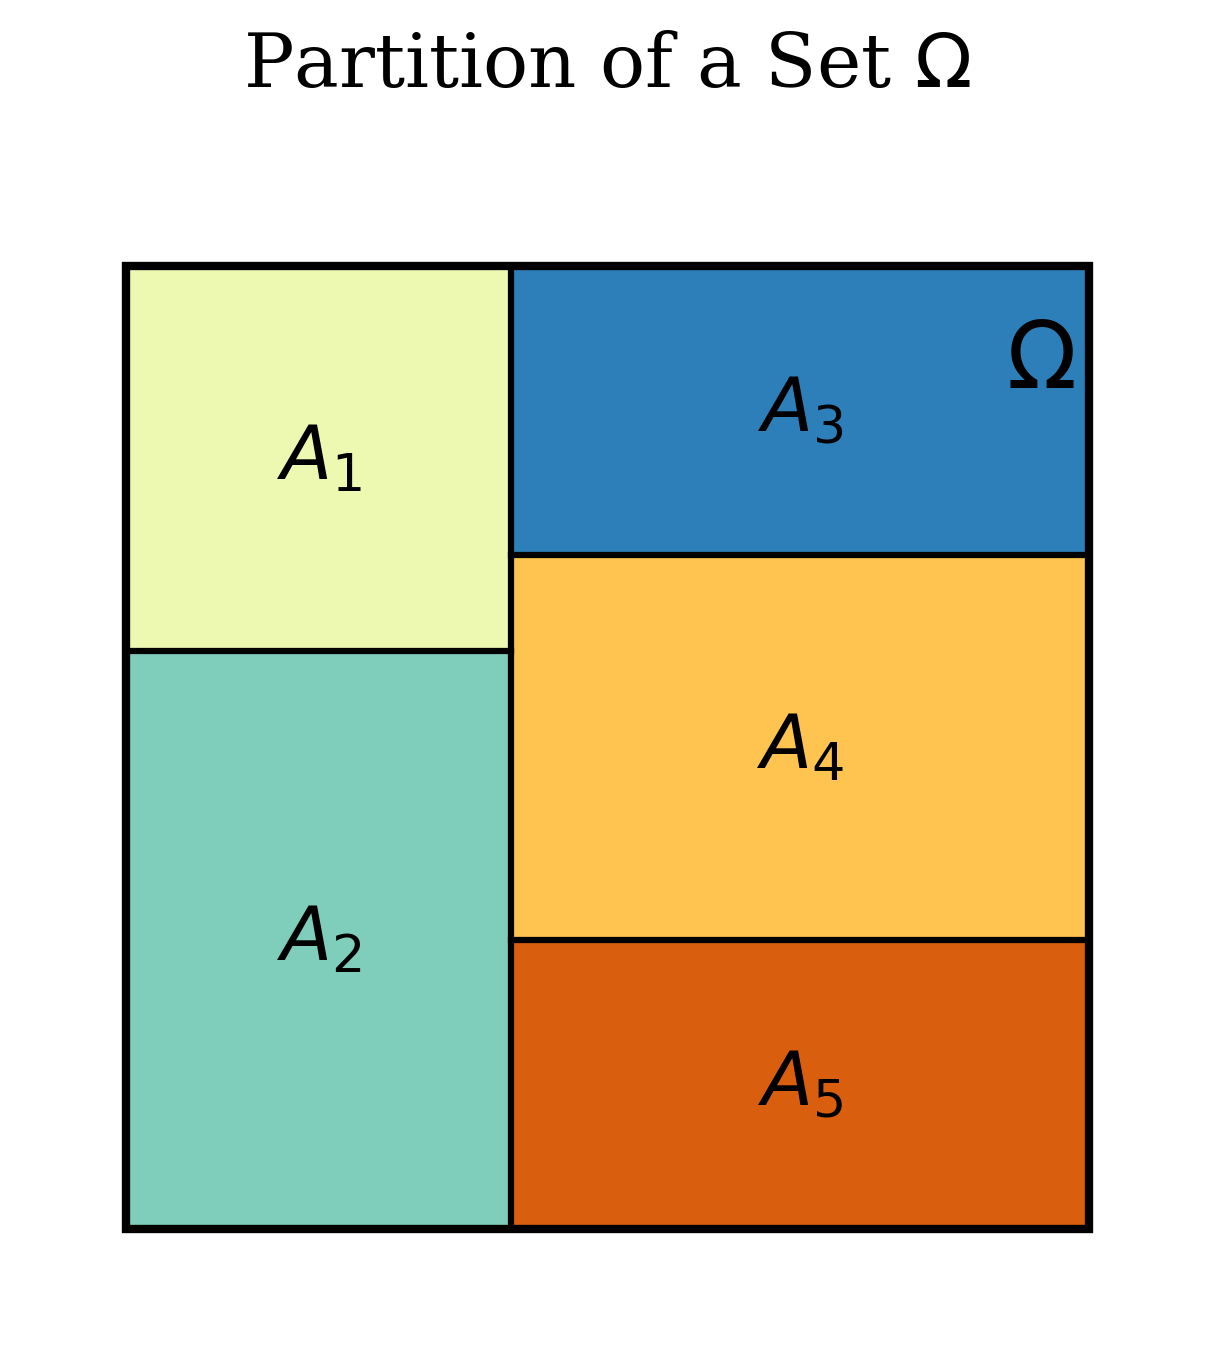
\includegraphics[width=0.6\textwidth]{figure_5_partition.png}
    \caption{A partition of the set $\Omega$ \cite{chan}.}
    \label{fig:partition_diagram}
\end{figure}

\subsection{Set Algebra Properties}
These properties are essential for manipulating sets.
\begin{itemize}
    \item \textbf{Commutative Laws:} $A \cup B = B \cup A$; $A \cap B = B \cap A$ \cite{faculty_set, chan}.
    \item \textbf{Associative Laws:} $A \cup (B \cup C) = (A \cup B) \cup C$; $A \cap (B \cap C) = (A \cap B) \cap C$ \cite{faculty_set, chan}.
    \item \textbf{Distributive Laws:} $A \cap (B \cup C) = (A \cap B) \cup (A \cap C)$; $A \cup (B \cap C) = (A \cup B) \cap (A \cup C)$ \cite{faculty_set, chan}.
    \item \textbf{De Morgan's Laws:} $(A \cup B)^c = A^c \cap B^c$; $(A \cap B)^c = A^c \cup B^c$ \cite{faculty_set, chan}.
\end{itemize}

% --- Section 2: Cardinality & Countability ---
\section{Cardinality and Countability}

Understanding the "size" of sets, especially infinite sets, is important for defining sample spaces.

\subsection{Equicardinality and Bijective Functions}

\begin{definition}[Equicardinal Sets]
    Two sets $A$ and $B$ are \textbf{equicardinal} (have the same cardinality) if there exists a \textbf{bijective function} $f: A \to B$ between them \cite{faculty_set, chan}.
\end{definition}

\begin{definition}[Bijective Function]
    A function $f: A \to B$ is \textbf{bijective} (or a one-to-one correspondence) if it is both:
    \begin{itemize}
        \item \textbf{Injective (One-to-One):} For every $a_1, a_2 \in A$, if $f(a_1) = f(a_2)$, then $a_1 = a_2$. (Distinct inputs map to distinct outputs) \cite{faculty_set}.
        \item \textbf{Surjective (Onto):} For every $b \in B$, there exists at least one $a \in A$ such that $f(a) = b$. (Every element in the codomain is mapped to) \cite{faculty_set}.
    \end{itemize}
\end{definition}

\begin{figure}[h!]
    \centering
    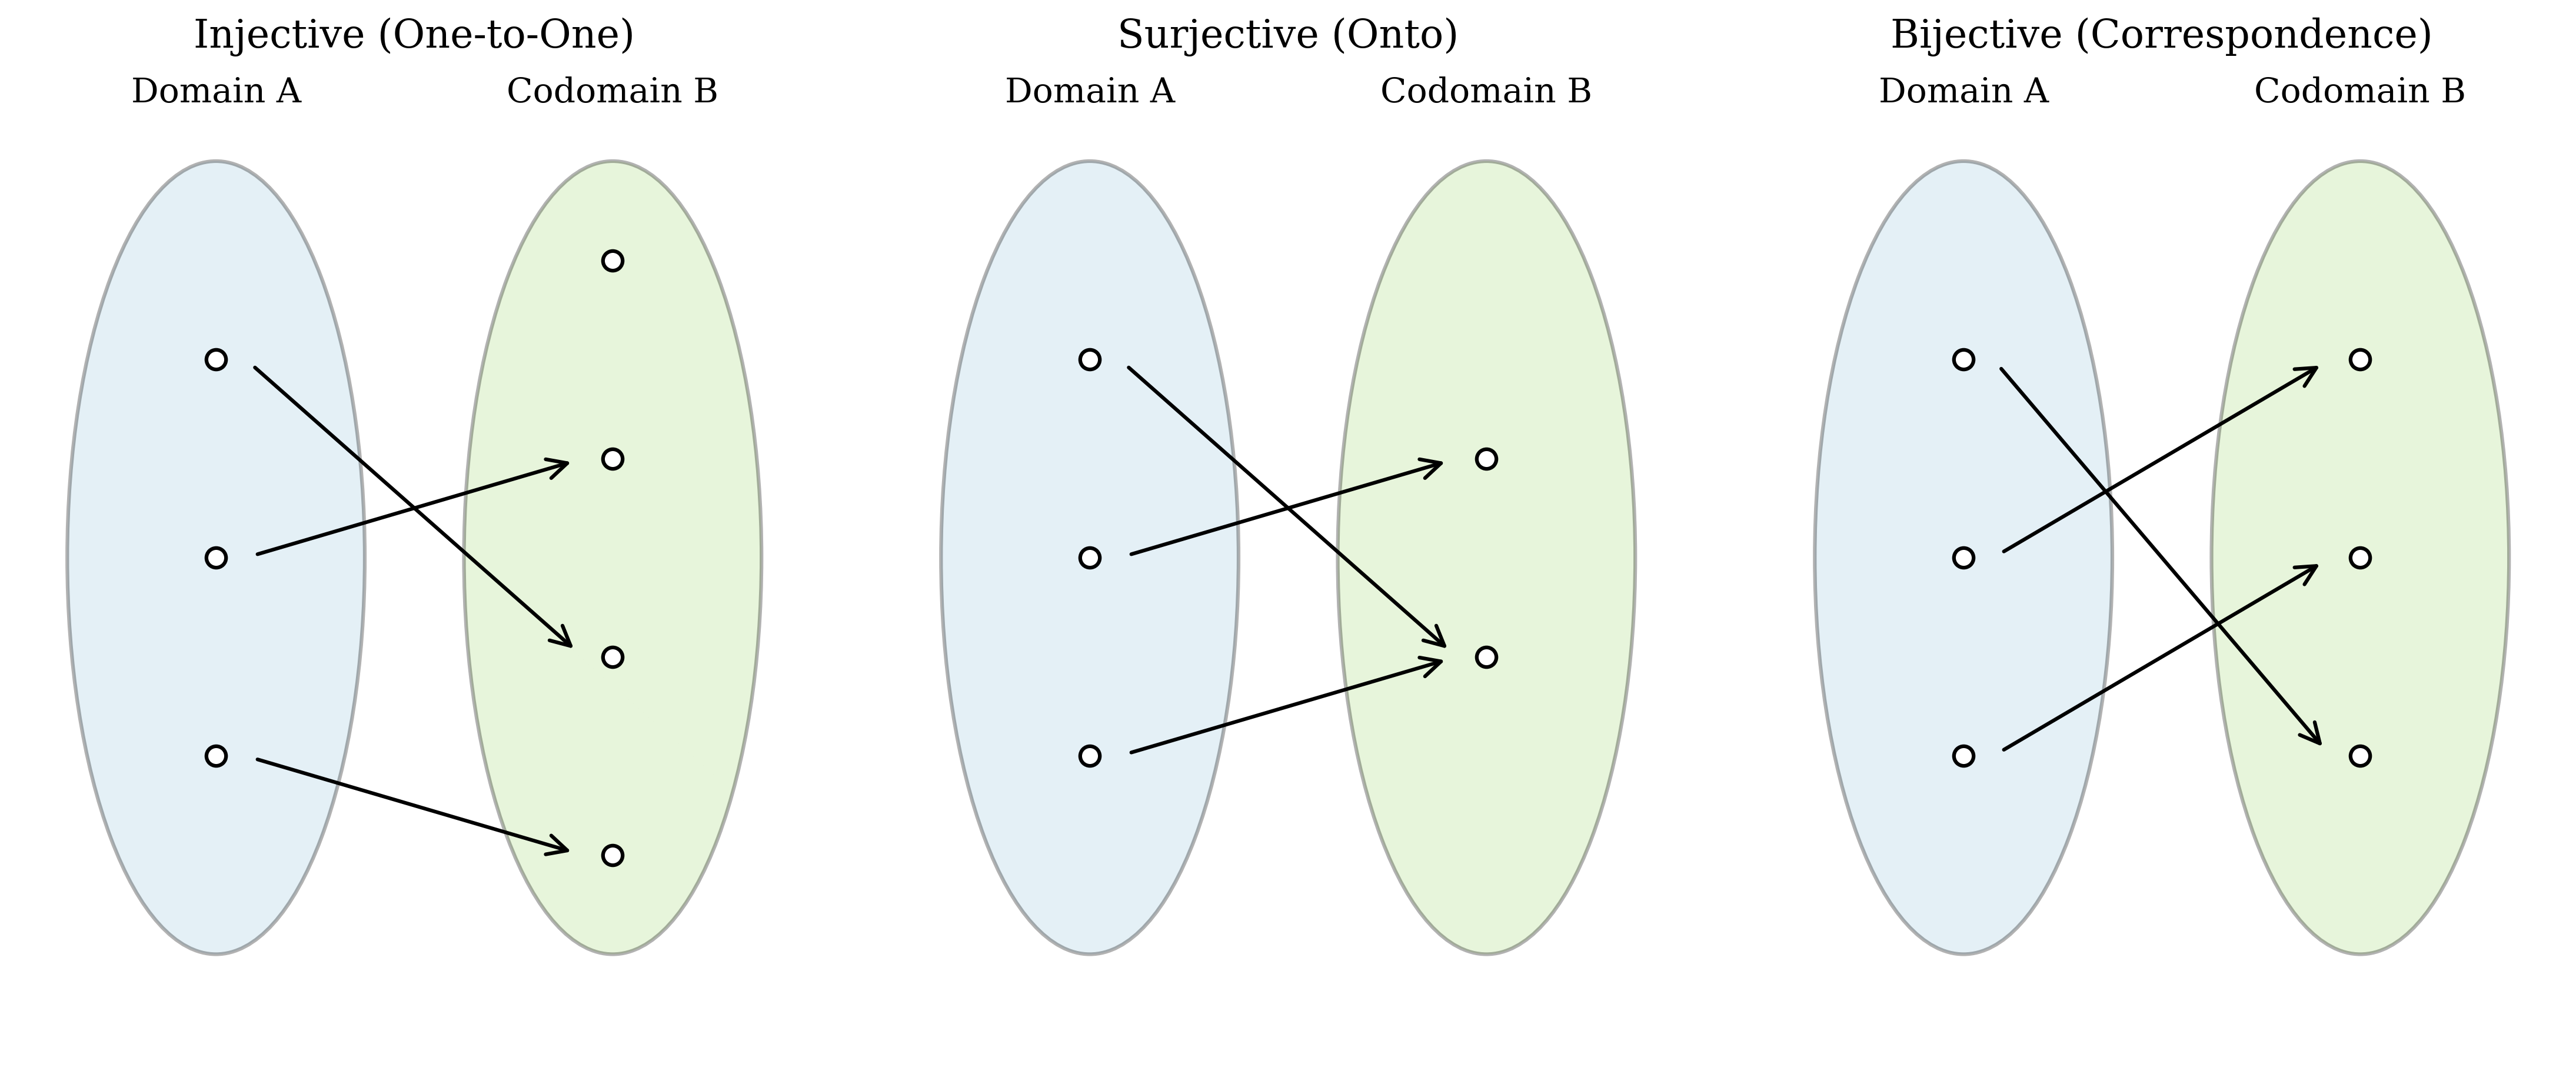
\includegraphics[width=0.9\textwidth]{figure_6_function_types.png}
    \caption{Illustrations of injective, surjective, and bijective functions.}
    \label{fig:function_types}
\end{figure}





\subsection{Types of Sets by Cardinality}

\begin{itemize}
    \item \textbf{Finite Set:} A set that is equicardinal with $\{1, 2, \dots, n\}$ for some non-negative integer $n$. Its cardinality is $n$ \cite{faculty_set}.
    \item \textbf{Infinite Set:} A set that is not finite \cite{faculty_set}.
        \begin{itemize}
            \item \textbf{Countably Infinite Set:} An infinite set that is equicardinal with the set of natural numbers $\mathbb{N} = \{1,2,3,\dots\}$ \cite{faculty_set, chan}.
            \item \textbf{Uncountable Set:} An infinite set that is not countably infinite \cite{faculty_set, chan}.
        \end{itemize}
\end{itemize}

\begin{definition}[Countable Set]
A set is \textbf{countable} if it is either finite or countably infinite \cite{chan}.
\end{definition}

\begin{example}
\begin{itemize}
    \item $\mathbb{N}$ (natural numbers), $\mathbb{Z}$ (integers), $\mathbb{Q}$ (rational numbers) are countable \cite{faculty_set, chan}.
    \item $\mathbb{R}$ (real numbers), intervals like $[0,1]$ or $(0,1)$ are uncountable \cite{faculty_set, chan}.
\end{itemize}
\end{example}

\begin{remark}
Every countably infinite set can be listed as a sequence.
\end{remark}

% Placeholder Figure: Countable vs Uncountable Sets
% Left: Enumeration arrows from N to elements in a set A (countable).
% Right: The interval [0,1] showing dense points (uncountable).
\begin{figure}[h!]
\centering
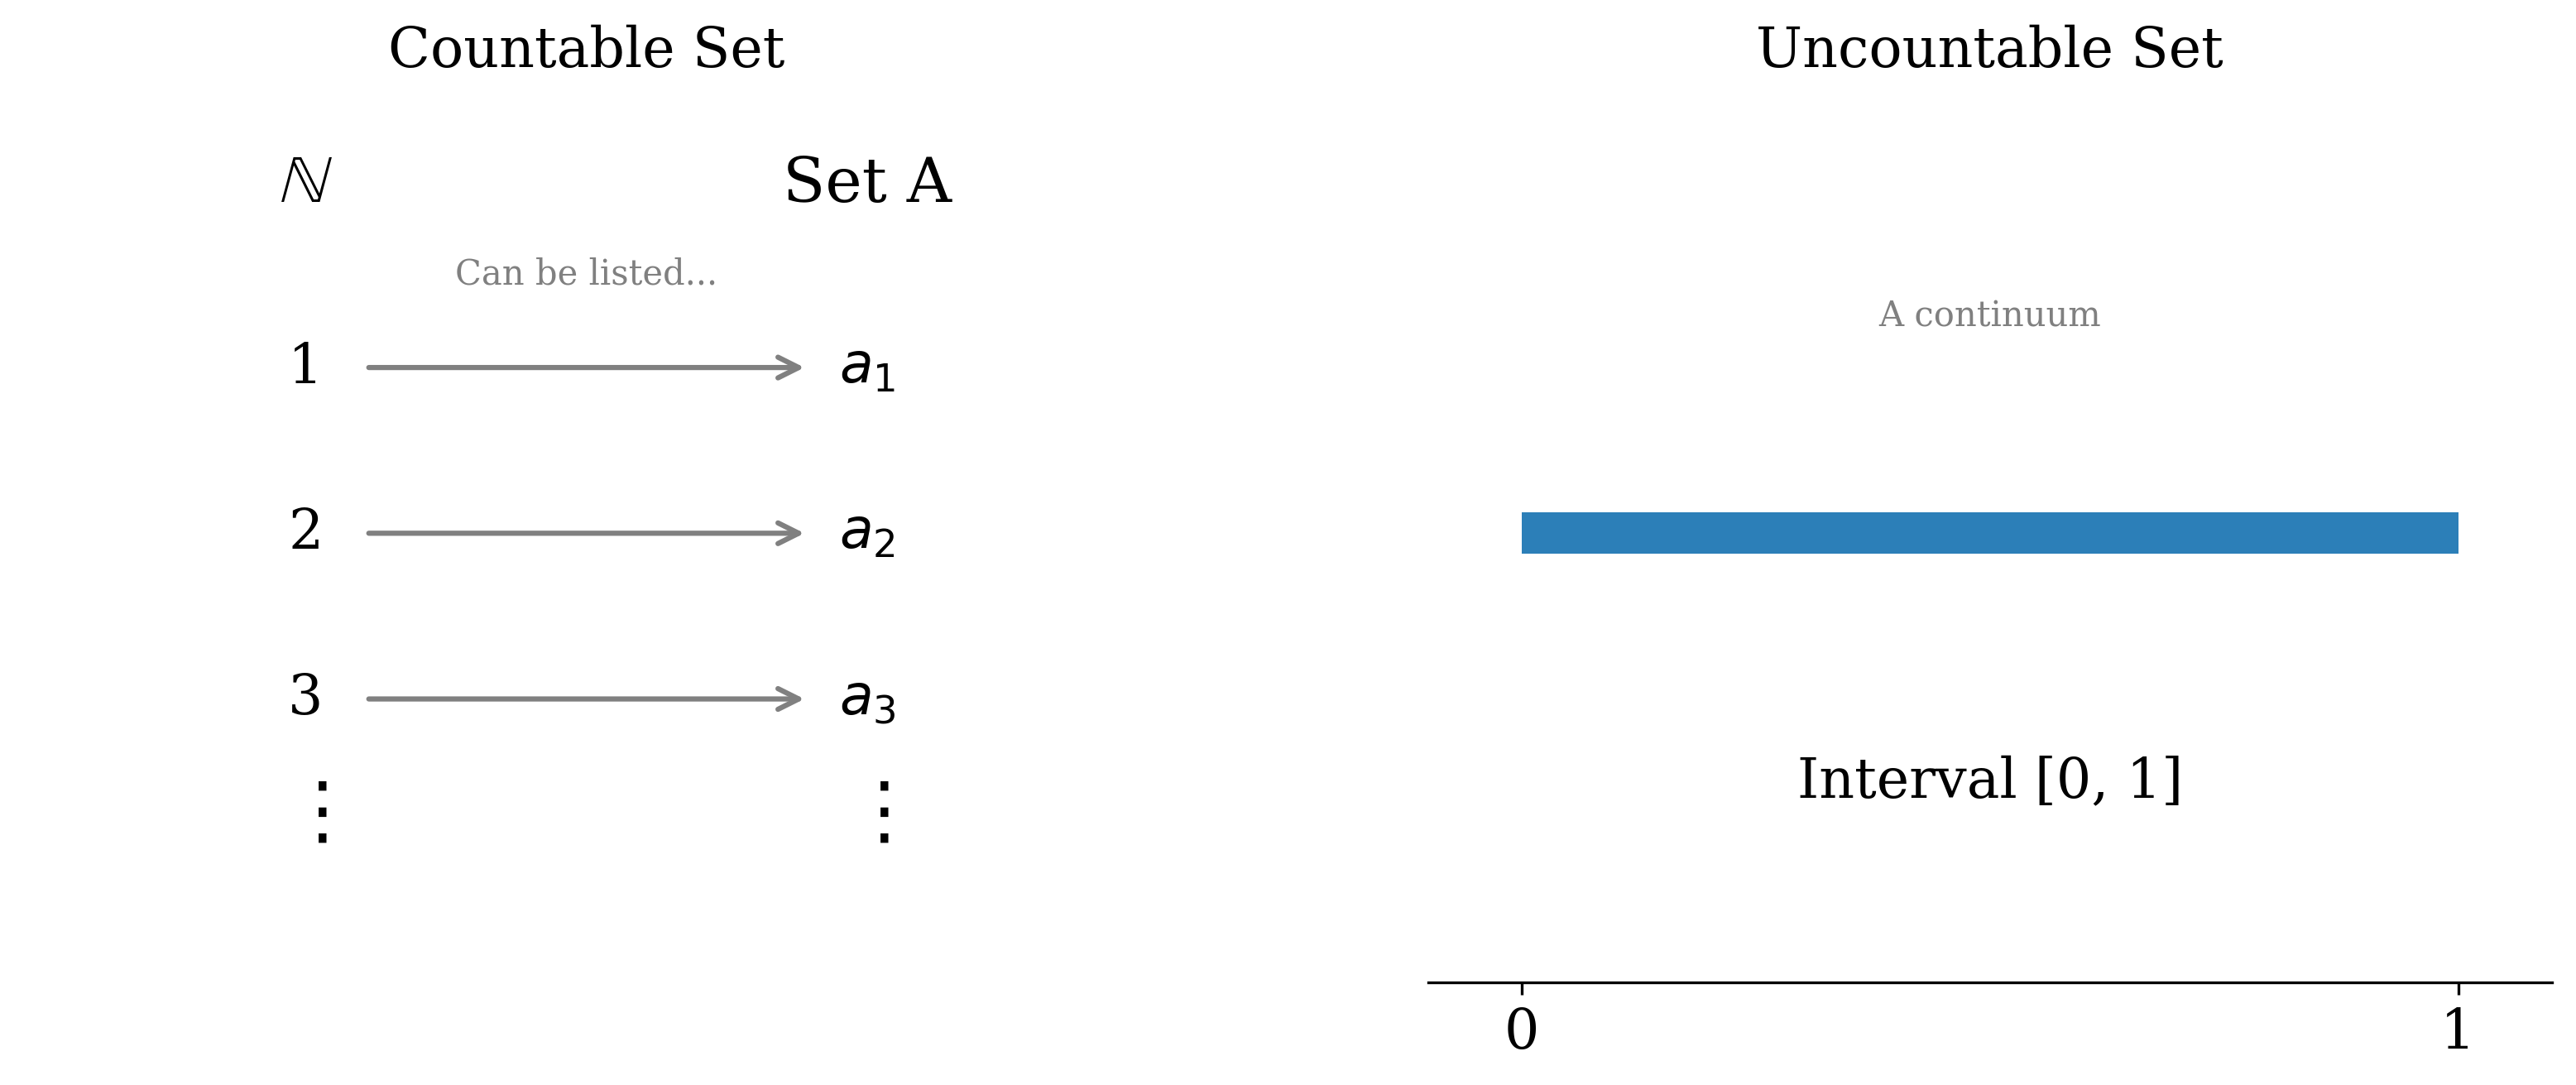
\includegraphics[width=0.9\textwidth]{figure_7_countability.png}
\caption{Visualization of countable and uncountable sets.}
\label{fig:countability}
\end{figure}


% --- Section 3: The Probability Space ---
\section{The Probability Space $(\Omega, \mathcal{F}, \mathbb{P})$}

Probability theory provides a mathematical framework for modeling experiments with random outcomes. This framework is the \textbf{probability space}, a triplet $(\Omega, \mathcal{F}, \mathbb{P})$ \cite{faculty_prob, chan}.

\subsection{Component 1: The Sample Space ($\Omega$)}

\begin{definition}[Sample Space]
    The \textbf{Sample Space} ($\Omega$) is the set of \emph{all possible outcomes} of a random experiment \cite{ross, chan}. Each outcome $w$ is an element of $\Omega$ ($w \in \Omega$). A sample space must be \textbf{exhaustive} (includes all possibilities) and its elements must be \textbf{mutually exclusive} (distinct outcomes) \cite{chan}.
\end{definition}

\begin{example}
    \begin{itemize}
        \item Experiment: Flip a coin. $\Omega = \{H, T\}$ \cite{ross}.
        \item Experiment: Roll a die. $\Omega = \{1, 2, 3, 4, 5, 6\}$ \cite{ross}.
        \item Experiment: Measure lifetime of a device. $\Omega = [0, \infty) = \{t \mid t \ge 0\}$ \cite{ross}.
    \end{itemize}
\end{example}

\subsection{Component 2: The Event Space ($\mathcal{F}$)}

\begin{definition}[Event]
    An \textbf{Event} ($A$) is a subset of the sample space ($\underline{A \subseteq \Omega}$) \cite{ross, chan}. An event is said to \textbf{occur} if the outcome of the experiment is an element of that event.
\end{definition}

\begin{example}
    Experiment: Roll a die, $\Omega = \{1, 2, 3, 4, 5, 6\}$.
    \begin{itemize}
        \item Event $A$: "An even number is rolled." $A = \{2, 4, 6\}$.
        \item Event $B$: "A number less than 3 is rolled." $B = \{1, 2\}$.
        \item Event $C$: "The number 5 is rolled." $C = \{5\}$.
    \end{itemize}
\end{example}

\begin{definition}[Event Space ($\sigma$-field)]
    The \textbf{Event Space} ($\mathcal{F}$) is a collection of subsets of $\Omega$ (i.e., a set of events) that satisfies the properties of a \textbf{$\sigma$-field} (or $\sigma$-algebra). This ensures that we can consistently assign probabilities and perform operations like complements and unions \cite{chan}.
    A collection $\mathcal{F}$ of subsets of $\Omega$ is a $\sigma$-field if:
    \begin{enumerate}
        \item $\Omega \in \mathcal{F}$ (The sample space itself is an event).
        \item If $A \in \mathcal{F}$, then $A^c \in \mathcal{F}$ (Closed under complementation).
        \item If $A_1, A_2, ... \in \mathcal{F}$ (a countable sequence), then $\bigcup_{i=1}^{\infty} A_i \in \mathcal{F}$ (Closed under countable unions).
    \end{enumerate}
\end{definition}

\begin{remark}
    For discrete sample spaces, $\mathcal{F}$ is usually the \textbf{power set} $P(\Omega)$ (the set of all subsets) \cite{faculty_set, chan}. For continuous spaces like $\mathbb{R}$, $\mathcal{F}$ is the \textbf{Borel $\sigma$-field} $B(\mathbb{R})$, generated by intervals \cite{faculty_prob, chan}.
\end{remark}

\subsection{Component 3: The Probability Law ($\mathbb{P}$)}

\begin{definition}[Probability Law/Measure]
    The \textbf{Probability Law} or \textbf{Probability Measure} $\mathbb{P}$ is a function that assigns a real number $\mathbb{P}[A]$ to each event $A \in \mathcal{F}$, satisfying the Axioms of Probability \cite{faculty_prob, chan}.
    $$\mathbb{P}: \mathcal{F} \rightarrow [0, 1]$$
    It quantifies the likelihood of each measurable event in $F$, serving as a measure of its relative size within the sample space \cite{chan}.
\end{definition}

\begin{figure}[h!]
    \centering
    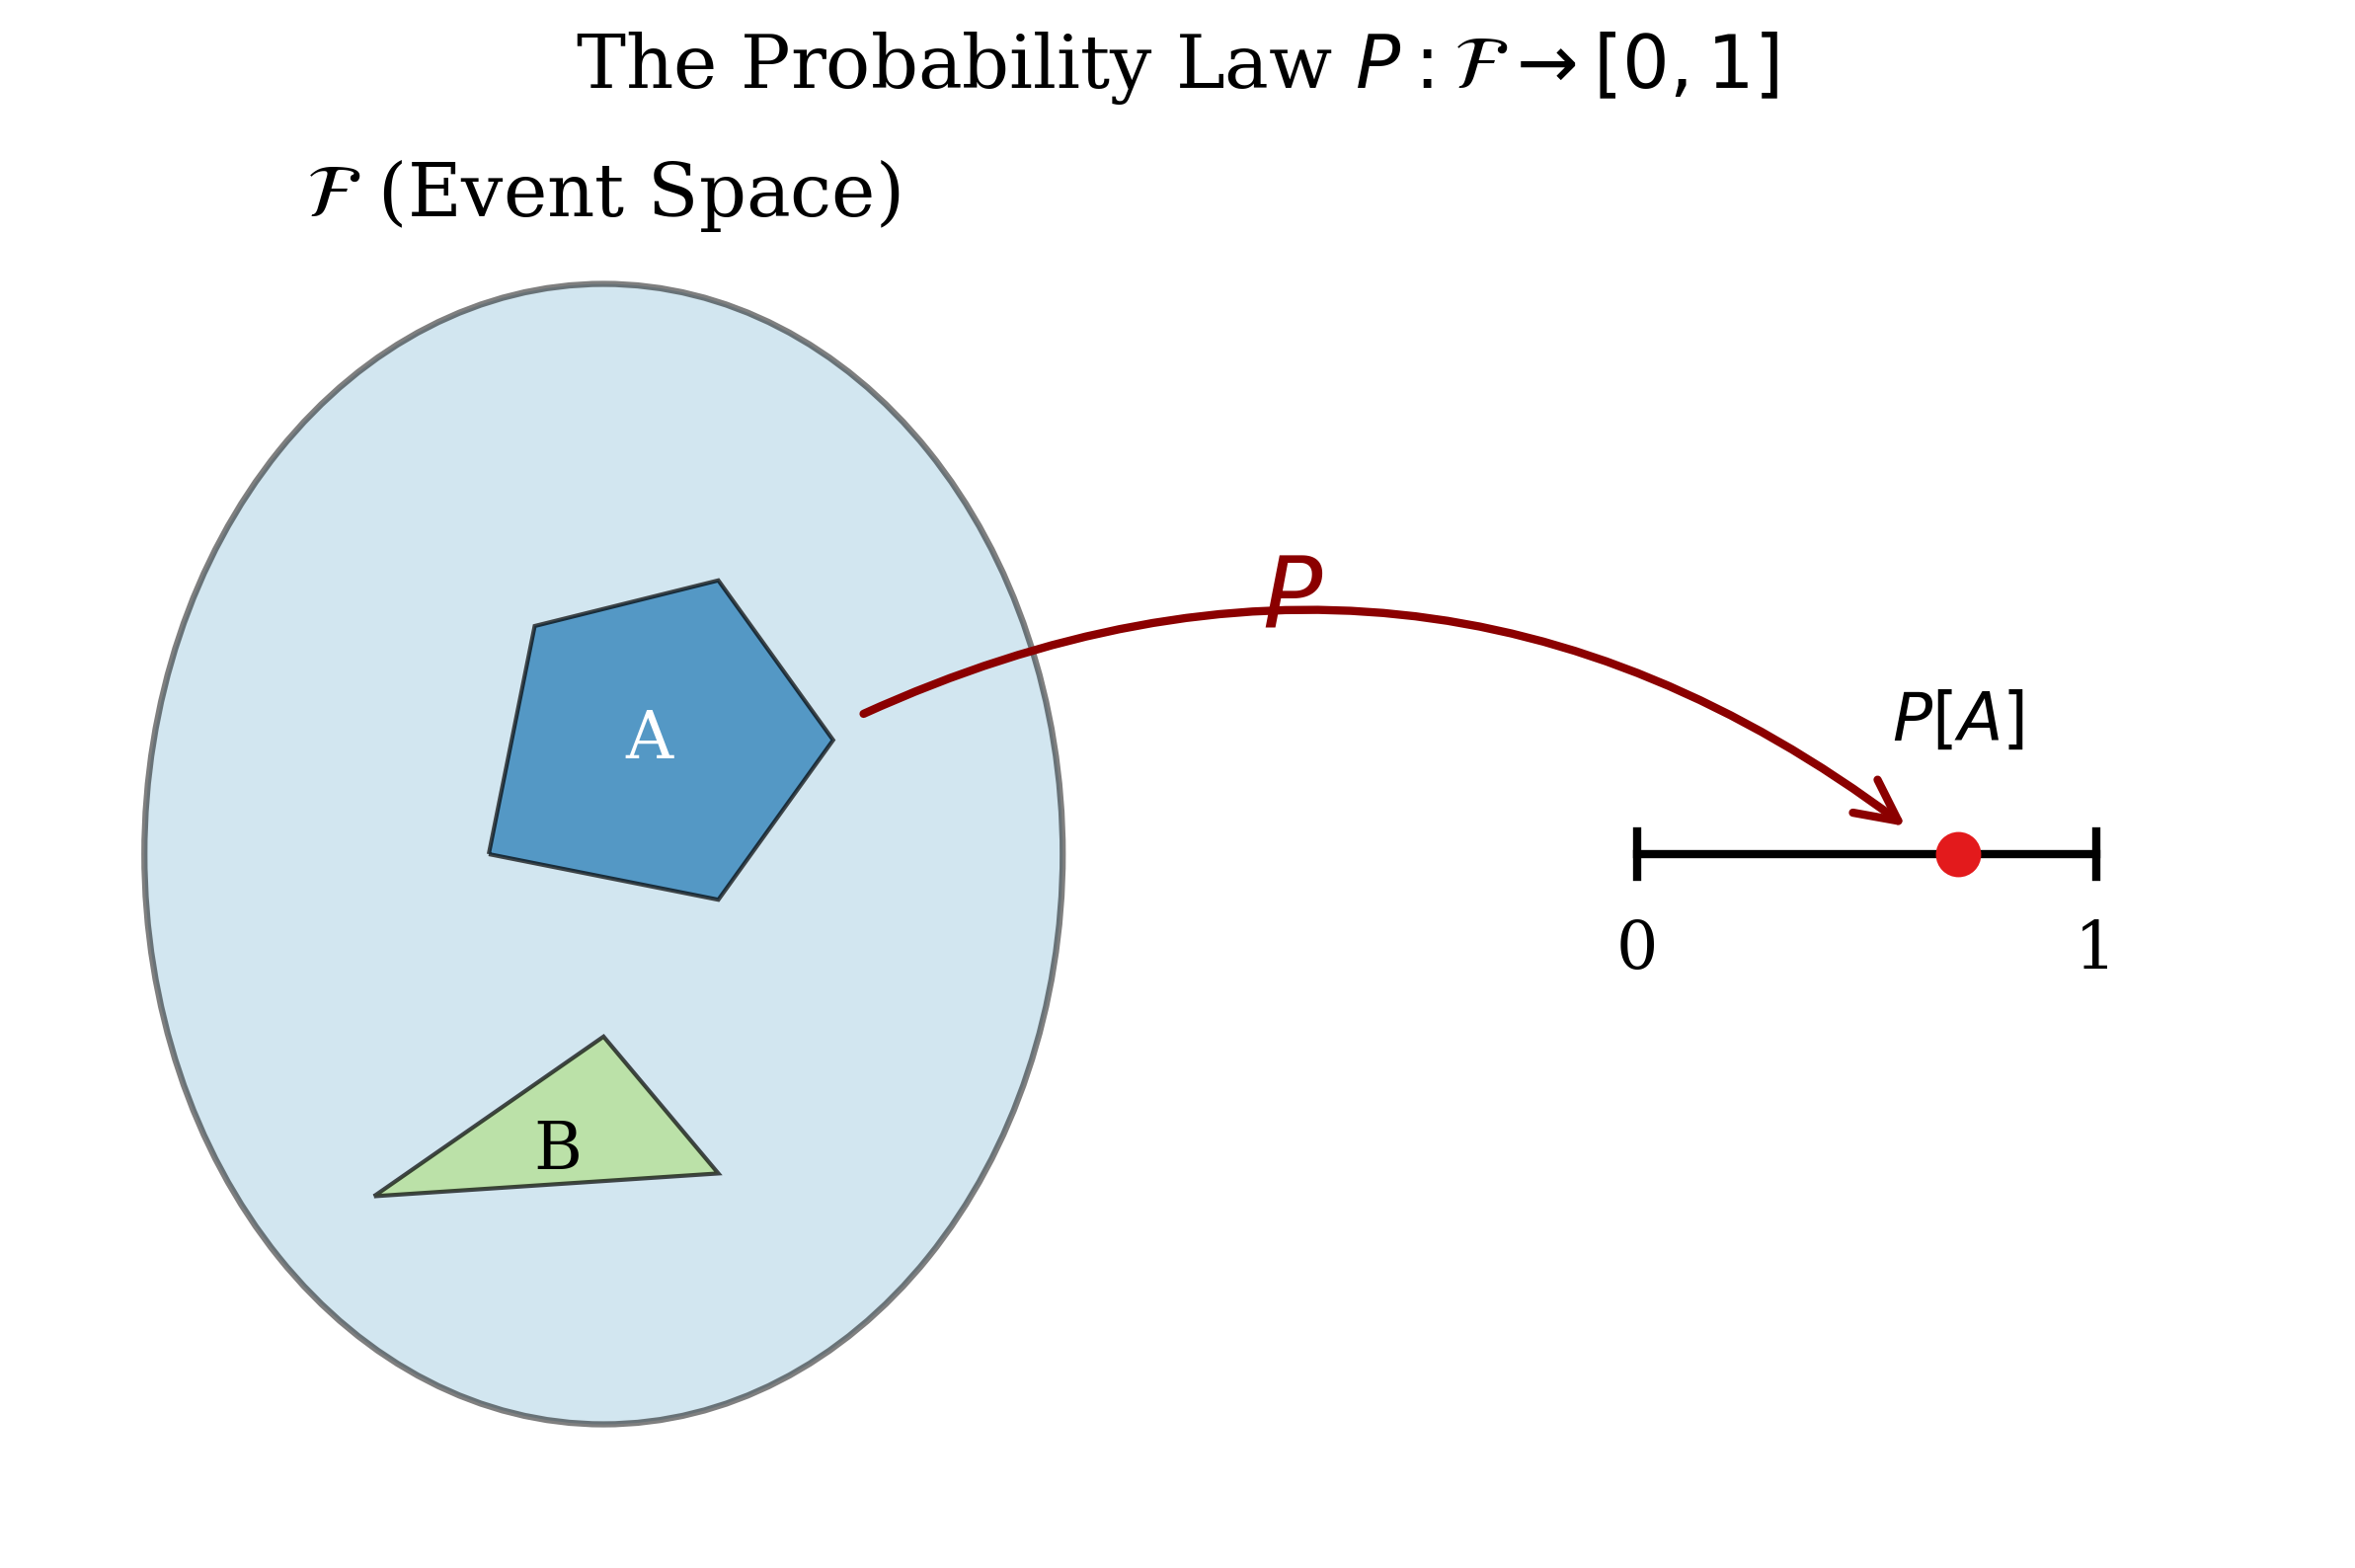
\includegraphics[width=0.6\textwidth]{figure_8_probability_law.png}
    \caption{The Probability Law $\mathbb{P}$ maps events from $\mathcal{F}$ to values in $[0, 1]$ \cite{chan}.}
    \label{fig:prob_map}
\end{figure}


\subsection{Measurable Sets and the Need for a $\sigma$-Field}

Not every subset of a sample space can be consistently assigned a probability. To avoid contradictions, probability is defined only on a specific collection of subsets \(F\) called a $\sigma$-field.

The sets in \(F\) are called \textbf{measurable sets}. A probability measure \(P\) assigns values only to these measurable events, not to arbitrary subsets \cite{chan}.

\begin{remark}
In continuous sample spaces such as \(\mathbb{R}\), the event space is usually the Borel $\sigma$-field \(\mathcal{B}(\mathbb{R})\), which contains intervals and any set formed from them using countable unions, intersections, and complements.
\end{remark}

\begin{example}
Every interval in \(\mathbb{R}\) such as \((0,1)\) or \([2,\infty)\) is measurable. However, there exist subsets of \(\mathbb{R}\) that are not measurable, and probability cannot be meaningfully assigned to them.
\end{example}

\begin{figure}[h!]
\centering
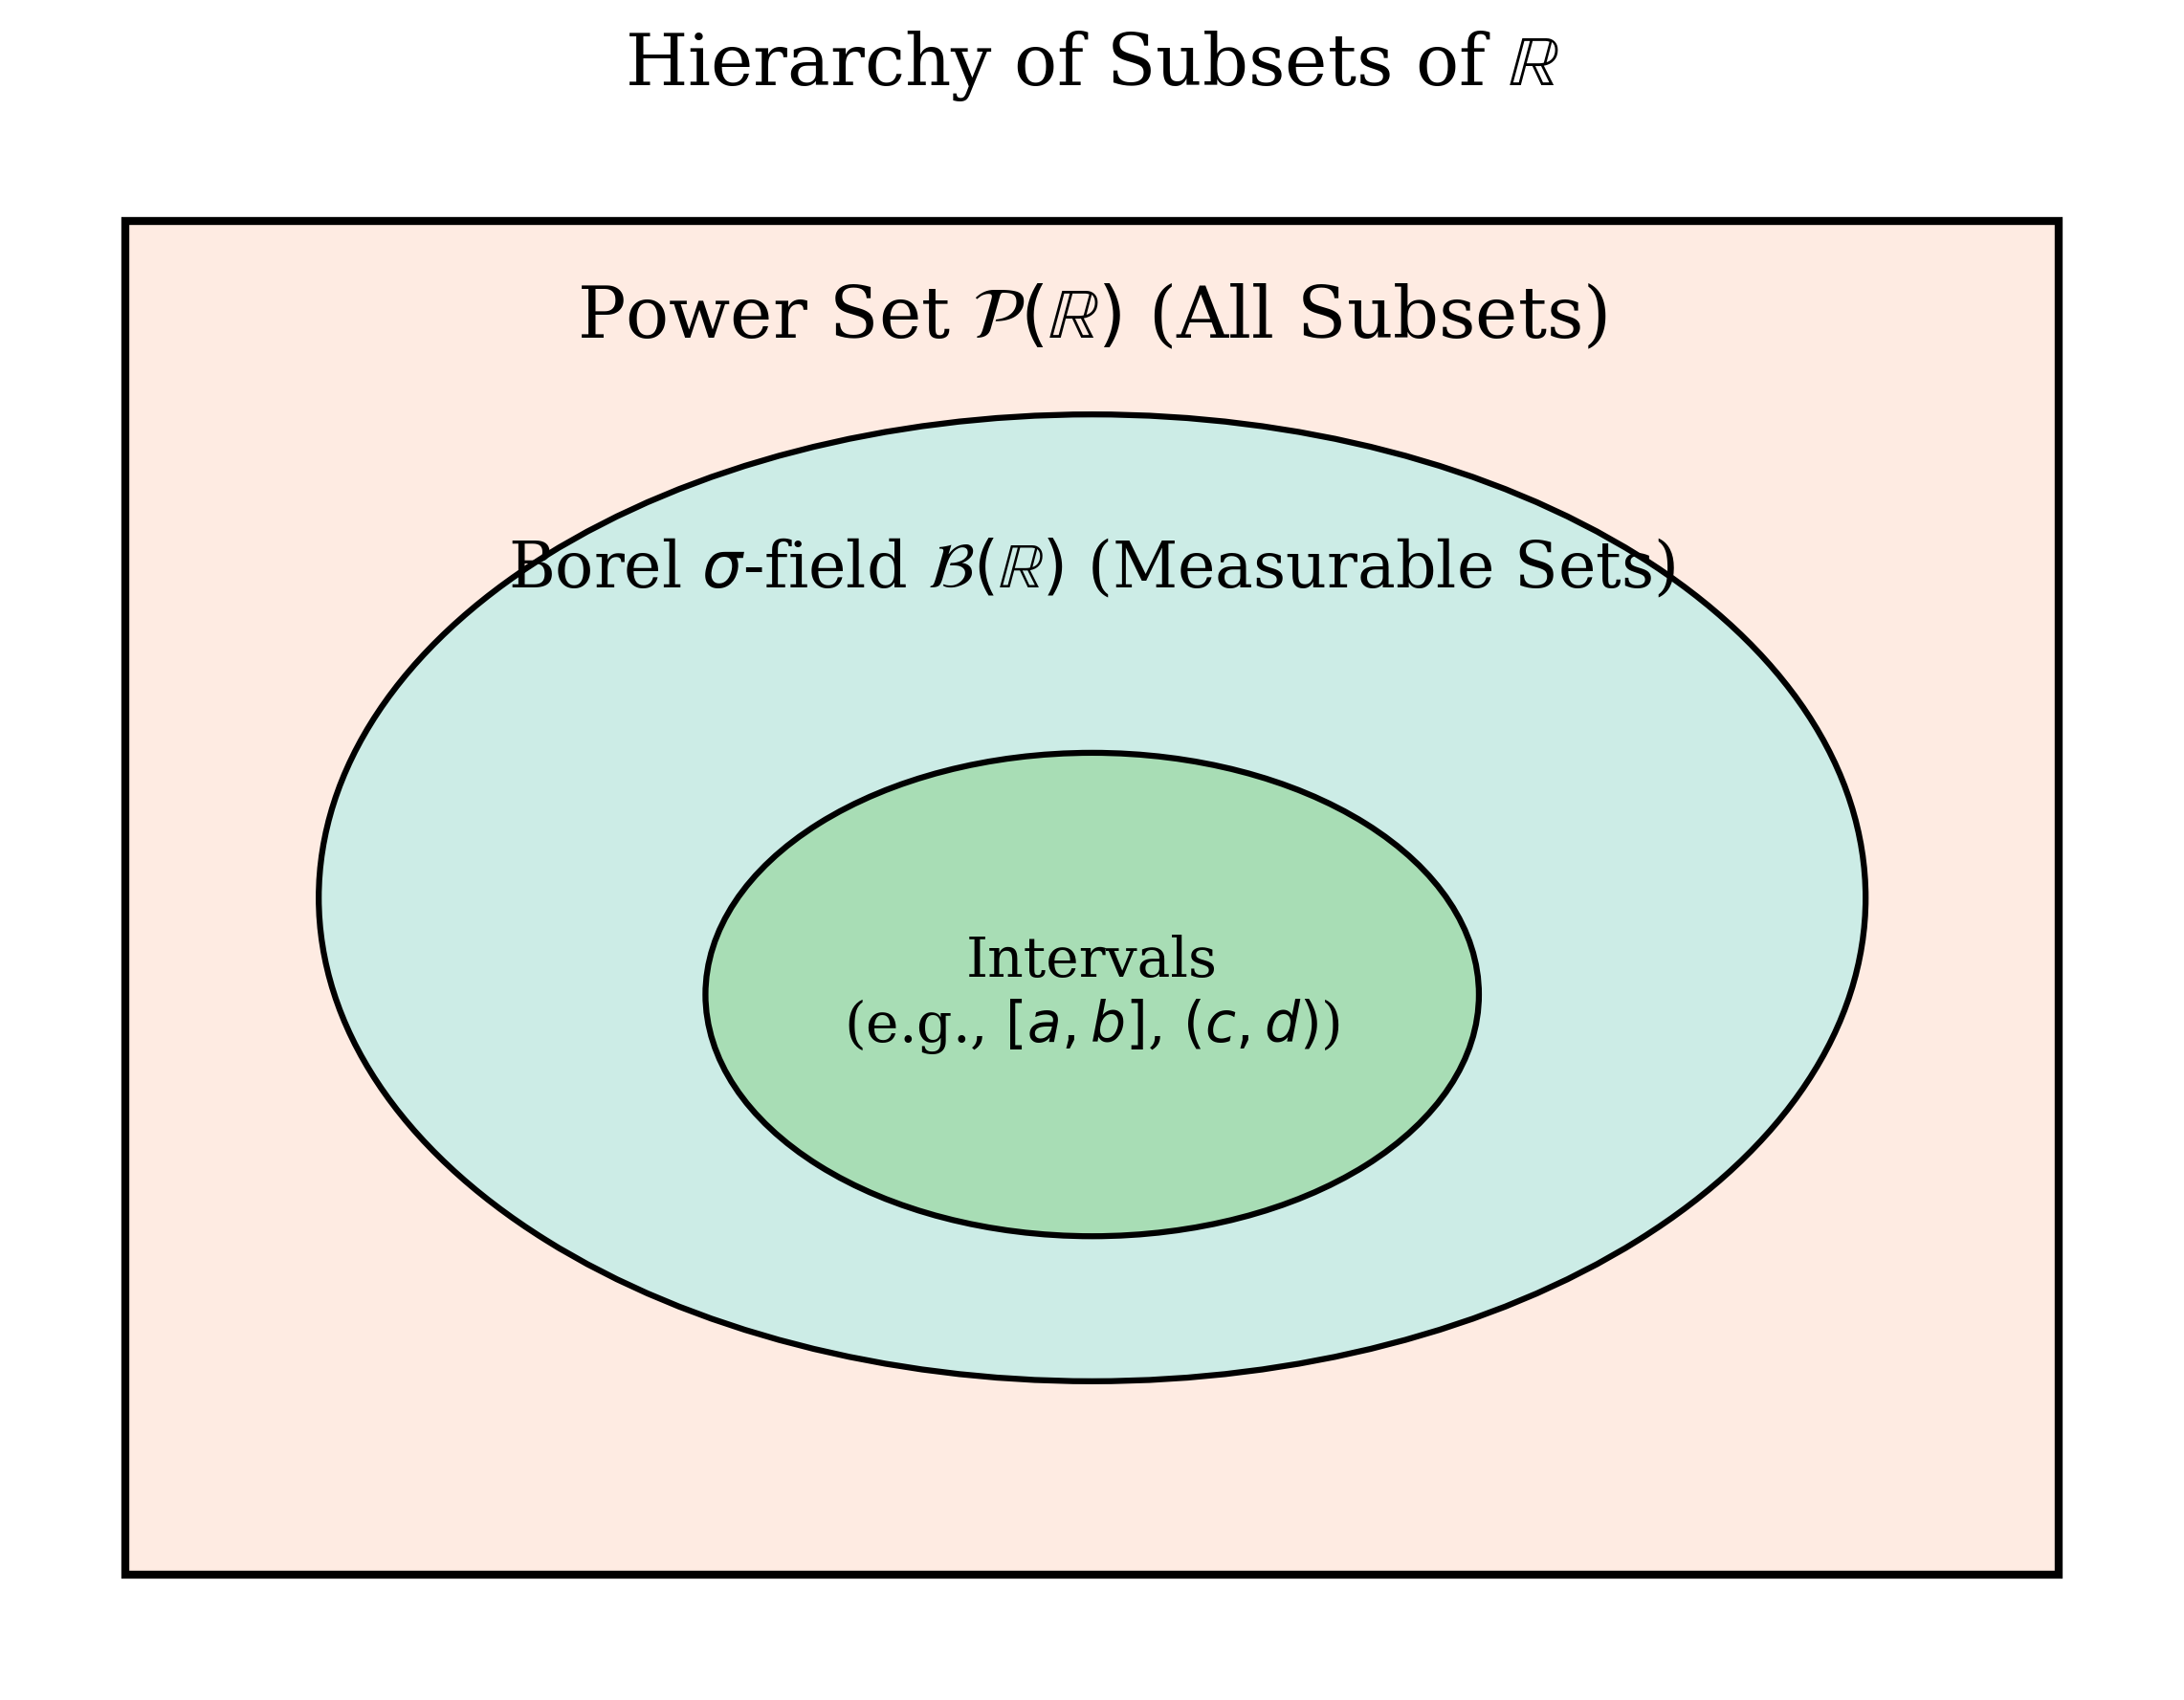
\includegraphics[width=0.6\textwidth]{figure_9_measurable_sets.png}
\label{fig:measurable_sets}
\end{figure}

Intuitively, probability measures the likelihood of measurable events. A $\sigma$-field ensures that this measurement behaves consistently.


% --- Section 4: Axioms ---
\section{The Axioms of Probability}

Any function $\mathbb{P}: \mathcal{F} \to [0, 1]$ must satisfy the following three axioms to be considered a valid probability measure \cite{ross, chan}.

\begin{enumerate}
    \item[\textbf{Axiom I}] \textbf{(Non-negativity):} For any event $A \in \mathcal{F}$,
        $$\mathbb{P}[A] \ge 0$$

    \item[\textbf{Axiom II}] \textbf{(Normalization):} The probability assigned to the entire sample space is 1.
        $$\mathbb{P}[\Omega] = 1$$

    \item[\textbf{Axiom III}] \textbf{(Countable Additivity):} For any countable sequence of \textbf{pairwise disjoint} events $\{A_1, A_2, ...\} \subseteq \mathcal{F}$ (i.e., $A_i \cap A_j = \emptyset$ for all $i \ne j$), the probability of their union is the sum of their individual probabilities.
        $$\mathbb{P}\left[\bigcup_{i=1}^{\infty} A_i\right] = \sum_{i=1}^{\infty} \mathbb{P}[A_i]$$
\end{enumerate}

\begin{remark}
    Axiom III implies \textbf{finite additivity}: For any finite collection of pairwise disjoint events $A_1, ..., A_n$,
    $$\mathbb{P}\left[\bigcup_{i=1}^{n} A_i\right] = \sum_{i=1}^{n} \mathbb{P}[A_i]$$
    In particular, for two disjoint events $A$ and $B$, $\mathbb{P}[A \cup B] = \mathbb{P}[A] + \mathbb{P}[B]$ \cite{chan}.
\end{remark}

% --- Section 5: Corollaries ---
\section{Corollaries from the Axioms}

These fundamental properties are direct consequences of the axioms.

\begin{corollary}[Probability of the Complement]
    For any event $A$, $\mathbb{P}[A^c] = 1 - \mathbb{P}[A]$ \cite{faculty_prob, ross, chan}.
\end{corollary}
\begin{proof}
    Since $A$ and $A^c$ form a partition of $\Omega$ (they are disjoint and $A \cup A^c = \Omega$), Axioms II and III (finite additivity) give:
    $1 = \mathbb{P}[\Omega] = \mathbb{P}[A \cup A^c] = \mathbb{P}[A] + \mathbb{P}[A^c]$. Rearranging yields the result.
\end{proof}

\begin{corollary}[Probability of the Empty Set]
    $\mathbb{P}[\emptyset] = 0$ \cite{faculty_prob, ross, chan}.
\end{corollary}
\begin{proof}
    Since $\emptyset = \Omega^c$, apply Corollary 1: $\mathbb{P}[\emptyset] = \mathbb{P}[\Omega^c] = 1 - \mathbb{P}[\Omega] = 1 - 1 = 0$.
\end{proof}

\begin{corollary}[Monotonicity]
    If $A \subseteq B$, then $\mathbb{P}[A] \le \mathbb{P}[B]$ \cite{chan}.
\end{corollary}
\begin{proof}
    We can write $B = A \cup (B \setminus A)$. The sets $A$ and $B \setminus A$ are disjoint. By Axiom III, $\mathbb{P}[B] = \mathbb{P}[A] + \mathbb{P}[B \setminus A]$. Since $\mathbb{P}[B \setminus A] \ge 0$ by Axiom I, it follows that $\mathbb{P}[B] \ge \mathbb{P}[A]$.
\end{proof}

\begin{corollary}[Inclusion-Exclusion Principle (for 2 events)]
    For \emph{any} two events $A$ and $B$:
    $$\mathbb{P}[A \cup B] = \mathbb{P}[A] + \mathbb{P}[B] - \mathbb{P}[A \cap B]$$ \cite{faculty_prob, ross, chan}
\end{corollary}
\begin{proof}
    We can write $A \cup B$ as the union of three disjoint sets: $(A \setminus B)$, $(B \setminus A)$, and $(A \cap B)$.
    Thus, $\mathbb{P}[A \cup B] = \mathbb{P}[A \setminus B] + \mathbb{P}[B \setminus A] + \mathbb{P}[A \cap B]$.
    Also, $A = (A \setminus B) \cup (A \cap B)$ (disjoint union), so $\mathbb{P}[A] = \mathbb{P}[A \setminus B] + \mathbb{P}[A \cap B]$, which implies $\mathbb{P}[A \setminus B] = \mathbb{P}[A] - \mathbb{P}[A \cap B]$.
    Similarly, $\mathbb{P}[B \setminus A] = \mathbb{P}[B] - \mathbb{P}[A \cap B]$.
    Substituting these into the first equation gives:
    $\mathbb{P}[A \cup B] = (\mathbb{P}[A] - \mathbb{P}[A \cap B]) + (\mathbb{P}[B] - \mathbb{P}[A \cap B]) + \mathbb{P}[A \cap B]$,
    which simplifies to $\mathbb{P}[A \cup B] = \mathbb{P}[A] + \mathbb{P}[B] - \mathbb{P}[A \cap B]$.
\end{proof}

% --- Section 6: Conditional Probability ---
\section{Conditional Probability}

Conditional probability allows us to update the probability of an event based on the knowledge that another event has occurred.

\subsection{Definition}

\begin{definition}[Conditional Probability]
    Given two events $A$ and $B$, with $\mathbb{P}[B] > 0$, the \textbf{conditional probability of $A$ given $B$} is defined as:
    $$\mathbb{P}[A \mid B] = \frac{\mathbb{P}[A \cap B]}{\mathbb{P}[B]}$$ \cite{faculty_prob}
\end{definition}

\begin{remark}
    Intuitively, knowing that $B$ has occurred restricts the relevant sample space to just the outcomes within $B$. $\mathbb{P}[A \mid B]$ measures the proportion of the probability mass within $B$ that also corresponds to outcomes in $A$.
\end{remark}

\subsection{Conditional Probability as a Valid Probability Measure}

For a fixed event $B$ with $\mathbb{P}[B] > 0$, the function $P_B(\cdot) = \mathbb{P}[\cdot \mid B]$ defines a new, valid probability measure on the original sample space $\Omega$ and event space $\mathcal{F}$. It satisfies the three axioms \cite{faculty_prob}.

\begin{proof} (Verifying the axioms for $P_B(\cdot)$)
\begin{enumerate}
    \item \textbf{Non-negativity:} For any event $A$, $\mathbb{P}[A \cap B] \ge 0$ (Axiom I for $\mathbb{P}$) and $\mathbb{P}[B] > 0$. Therefore, $P_B(A) = \frac{\mathbb{P}[A \cap B]}{\mathbb{P}[B]} \ge 0$.
    
    \item \textbf{Normalization:} We need to show $P_B(\Omega) = 1$.
    $P_B(\Omega) = \mathbb{P}[\Omega \mid B] = \frac{\mathbb{P}[\Omega \cap B]}{\mathbb{P}[B]}$. Since $B \subseteq \Omega$, $\Omega \cap B = B$. Thus, $P_B(\Omega) = \frac{\mathbb{P}[B]}{\mathbb{P}[B]} = 1$.
    
    \item \textbf{Countable Additivity:} Let $A_1, A_2, ...$ be a sequence of pairwise disjoint events. We need to show $P_B(\bigcup A_i) = \sum P_B(A_i)$.
    \begin{align*}
        P_B\left(\bigcup_{i=1}^{\infty} A_i\right) &= \mathbb{P}\left[\bigcup_{i=1}^{\infty} A_i \;\middle|\; B\right] \\
        &= \frac{\mathbb{P}\left[\left(\bigcup_{i=1}^{\infty} A_i\right) \cap B\right]}{\mathbb{P}[B]} \\
        &= \frac{\mathbb{P}\left[\bigcup_{i=1}^{\infty} (A_i \cap B)\right]}{\mathbb{P}[B]} \quad \text{(Distributive Law)}
    \end{align*}
    Since $A_i$ are disjoint, the events $(A_i \cap B)$ are also disjoint. Applying Axiom III for $\mathbb{P}$:
    \begin{align*}
        P_B\left(\bigcup_{i=1}^{\infty} A_i\right) &= \frac{\sum_{i=1}^{\infty} \mathbb{P}[A_i \cap B]}{\mathbb{P}[B]} \\
        &= \sum_{i=1}^{\infty} \frac{\mathbb{P}[A_i \cap B]}{\mathbb{P}[B]} \\
        &= \sum_{i=1}^{\infty} \mathbb{P}[A_i \mid B] = \sum_{i=1}^{\infty} P_B(A_i)
    \end{align*}
\end{enumerate}
Thus, $P_B(\cdot)$ is a valid probability measure.
\end{proof}

% --- Bibliography ---
\newpage
\bibliographystyle{plain} % Simple citation style
\bibliography{references} % Points to the references.bib file

\end{document}